%++++++++++++++++++++++++++++++++++++++++
% Don't modify this section unless you know what you're doing!
\documentclass[letterpaper,10pt]{article}
\usepackage{tabularx} % extra features for tabular environment
\usepackage{textcomp}
\usepackage{gensymb}
\usepackage{amsmath}  % improve math presentation
\usepackage{graphicx} % takes care of graphic including machinery
\usepackage{subfig}
\usepackage{wrapfig}
\usepackage{xcolor}
\usepackage{rotating}
\usepackage[margin=1in,letterpaper]{geometry} % decreases margins
\usepackage{cite} % takes care of citations
\usepackage[final]{hyperref} % adds hyper links inside the generated pdf file
\hypersetup{
	colorlinks=true,       % false: boxed links; true: colored links
	linkcolor=blue,        % color of internal links
	citecolor=blue,        % color of links to bibliography
	filecolor=magenta,     % color of file links
	urlcolor=blue         
}
%++++++++++++++++++++++++++++++++++++++++
\graphicspath{{/home/clay/Documents/research/jgr20/manuscript/plots/}}

\begin{document}

%\title{The Effect of Roughness on the Elasticity and Permeability of Fractured Media}
%\author{C. Wood, B. Madera, P. Shokouhi, J. Jin, J. Rivi\`{e}re, D. Elsworth, C. Marone}
%%\date{\today}
%\maketitle

\section{Possible Titles}
\begin{flushleft}
	\begin{Large}
	\textbf{The effect of roughness on the elasticity and permeability of fractured media
	\linebreak\linebreak\linebreak
	The relation between changes in permeability and elastic wave velocity in dynamically stressed fractured rocks
	\linebreak\linebreak\linebreak
	The relation between \textit{transient} changes in permeability and elastic wave velocity in dynamically stressed fractured rocks
	\linebreak\linebreak\linebreak
	Elastodynamic and poromechanical properties of fractured rock
	\linebreak\linebreak\linebreak
	Characterizing the elastodynamic and poromechanical properties of fractured rock with dynamic stressing}
\end{Large}
\end{flushleft}
\pagebreak


\section{Abstract}
We describe laboratory work to elucidate the relationship between nonlinear elasticity and
permeability of fractured media subjected to local stress perturbations in relation to fracture
roughness and aperture distribution. This study is part of an effort to image fluid pathways and
fracture properties using locally induced seismicity, associated with fluid injection. Experiments were conducted in which intact L-shaped Westerly Granite samples were fractured in-situ tri-axial conditions while forcing deionized water through the subsequent fracture interfaces. After in-situ fracture, we imposed oscillations of the applied Normal stress and pore pressure with amplitudes ranging from 0.2 to 1 MPa and frequencies from 0.1 to 10 Hz. During these dynamic perturbations an array of ultrasonic transducers (PZTs) continuously generated and transmitted p-wave pulses to monitor the elastic response of the granite samples. We interpret the relative change in p-wave velocities to be an analog for the elastic non-linearity and relate it to the permeability of the fractured media. The roughness of the fracture interfaces is altered during experiments by shearing the L-shaped samples and then allowing the interface to age before applying dynamic stressing. We observe changes in the permeability and stiffness of the fracture during the dynamic perturbations and also with the shearing history, changing roughness, of the Westerly Granite samples.

\pagebreak
\section{Introduction}
%\textcolor{red}{As you yourself have noted, this is very similar to GRL’s introduction and needs to be re-written.}\\
%\textcolor{red}{We will need to include a paragraph (w relevant literature) discussing how shearing changes nonlinearity.}\\

\paragraph{} Dynamic stresses associated with energy production and waste water sequestration (injection, pumping, and transport of supercritical $H_{2}O$--$CO_{2}$ fluids) are particularly concerning as they are known to induce seismicty [Healy et al., 1968; Raleigh et al., 1976; Simpson et al., 1988; Sminchak and Gupta, 2003; McNamara et al., 2015; McGarr et al., 2015; Walsh and Zoback, 2015]. 

\paragraph{} Though dynamic stressing could be beneficial for enhanced permeability, it presents a significant risk associated with fault reactivation, reservoir seal damage, and accelerated deformation. Therefore, it is important to understand how fluid injection influences the hydromechanical properties of rocks and fractures. We have performed careful laboratory experiments to investigate the connection between fluid flow and elastic nonlinearity (i.e. stress is not proportional to strain) of fractured media.

\paragraph{} Dynamic stressing of the local subsurface associated with seismicity, drilling, hydraulic injection cause transient changes in permeability. These perturbations cause significant changes in the local stress field and consequently the poromechanical properties of the local subsurface. Empirical evidence from the field and laboratory show that earthquakes and subsequent seismic waves cause transient changes in rock stiffness in the proximity of faults. Specifically, measurements of a sudden decrease in seismic wave velocity from co-seismic softening and a post-seismic relaxation of the rock stiffness, a logarithmic recovery in time. Scaling down to laboratory studies, it has been shown that by using dynamic acousto-elastic testing, ultrasonic wave velocity (analog for field-scale seismometers) recorded decreased during dynamic stressing and then recovered after dynamic stressing ended with a logarithmic form. Dynamic perturbations with strain on the order of $10^{-6}$ cause a transient decrease in stiffness in nonlinear elastic materials. 
%\textit{It would be nice to mention any studies b/w lab- and field-scale.} 

\paragraph{} Anthropogenic activities on the field-scale such as drilling, wastewater storage, hydraulic fracturing result in considerable deformation of reservoir rocks. Changing the hydromechanical properties by dynamic stressing from fluid injection are likely to present hazards in the form of fault reactivation and reservoir seal damage. Evidence of this type of stressing inducing regional seismicity is rich and numerous (\textit{more details and citations}). Despite the hazards, dynamic stressing of the subsurface may result in enhanced permeability, consequently greater energy recovery. 
Seismic and anthropogenic sources of dynamic perturbation both change rock stiffness and permeability in similar ways, which suggests there is a physical mechanism that relates the nonlinear stiffness and poromechanical properties of fractured rock.

\paragraph{} Nonlinear response is sensitive to many fracture properties: geometry, flow pathways, asperity compliance, and friction. Currently, literature for investigating the relationship b/w elastodynamic and poromechanical and subsequent recovery is quite limited. We present the results from sophisticated well-controlled laboratory experiments in which we combine the analysis of nonlinear elastodynamic and hydraulic data. 

\paragraph{} It is expected that the nonlinear behavior of rocks is sensitive to fine features such as fracture aperture (i.e. flow pathways, asperity stiffness). In order to fully under-stand the ramifications of dynamic stressing in the subsurface, we need elucidate the relationship between the elastodynamic and hydro-mechanical properties of fractured rocks. 


\pagebreak

\section{Experimental Setup}

\paragraph{} We conducted sophisticated experiments in which samples were loaded under triaxial conditions inside a pressure vessel and fractured in-situ to simultaneous measure flow rate and elastic properties. Westerly granite samples were prepared by cutting them into L-shape blocks (69 x 45 50 x 26 mm, Figure \ref{fig:samplesetup}) with 3 mm deep notches on the top and bottom to ensure reproducibility of planar fracture propagation. The L-shape is used for maintaining constant nominal contact area during fracture and shear. The samples were saturated in deionized water and then placed between steel forcing blocks that have embedded piezoelectric transducers. The P-polarized lead-zirconate transducers (PZTs) of company APC International Ltd. are 6.5 mm in diameter, with a center frequency of 500 kHz and the spacing between the steel loading platen and the PZTs is 4mm. The shorter forcing block additionally contains internal conduits to provide fluid flow along the fracture plane. Deionized water was pumped through these narrow channels (45 x 1 mm) and covered by sintered porous fits and fed by five 1.6 mm diameter holes. Sintered porous frits (permeability ~ $10^{-14}$ $m^2$) are press-fit into cavities within the short forcing block to allow homogenous distribution of fluid. After securing this Single Direct Shear (SDS) configuration, it was sealed inside a latex jacket to separate confining and pore fluids. Fully prepared and jacketed samples were fitted inside a pressure vessel within a biaxial loading apparatus.

\paragraph{} The Biax consists of two hydraulic pistons capable of applying vertical and horizontal loads in displacement or load control. Forces are measured using custom-built, beryllium-copper strain-gauge load cells mounted on each loading piston. The load cells have an amplified output of ±5 V with an accuracy of ±5 N and are calibrated with a Morehouse proving-ring. Displacements are measured with direct-current displacement transducers (DCDT), with an accuracy of $\pm$ 0.1 $\mu m$. The confining fluid, a food-grade heat transfer oil (XCELTHERM 600, Radco Industries), in the sealed pressure vessel is pressurized to create a true-triaxial stress conditions. A linear variable differential transformer was attached to the outside of the sample, inside the pressure vessel, to accurately ($\pm 0.1\ \mu m$) measure the fracture displacement. Pressure intensifiers fitted with LVDTs and pressure transducers were used to control the confining pressure and the internal upstream and downstream pressures. 

\paragraph{} Each axis of loading is independently servo-controlled and all stresses, strains, fluid pressures and fluid volumes were recorded with $\pm10$ V, 16-channel 24-bit analog-to-digital converter at 10 kHz and averaged to sampling rates of 100 Hz or 1 kHz. Fracture permeability was measured using upstream and downstream pore-pressure intensifiers. Active ultrasonic data were recorded using a Vantage\textsuperscript{TM}\ Research Ultrasound (Verasonics) system. We use broadband (~0.02-2 MHz) PZTs (APC International Ltd. 6.35 diameter compressional crystals), which were successively pulsed every 1 ms on the transmitting side and the recording rate at the receiver side was 25 MHz. The input signal is a half sine with a frequency of 500 kHz. Also, a pulse from the Verasonics system accompanied the PZT excitation and is recorded by the 24-bit analog-to-digital data acquisition system. This allows us to sync the “ultrasonic” to “poro-mechanical” data and then analyzed to measure changes in the permeability and elasticity of the fractured rock samples, explained more fully in the signal analysis procedure.
  
\paragraph{} Before commencing each experiment, the samples were installed in the pressure vessel and then the vessel was sealed and then filled with confining fluid. A horizontal load of 20 MPa was applied and then the confining fluid pressure was slowly increased to 15 MPa; it is important to monitor the integrity sample jacket seal during this step. Next, we applied a pore pressure differential: inlet ($P_{pA}$ = 4 MPa) and outlet ($P_{pB}$ = 2 MPa). At this point there was no flow because Westerly granite matrix permeability is very low ($< 10^{-20}\ m^2$) and the confining fluid pressure is greater than the pore pressure (there was no flow around the sample). After establishing all loads and pore pressure, the ultrasonic data acquisition Once all fluid pressures and solid stresses were applied, the ultrasonic data acquisition system (Verasonics\textsuperscript{\textregistered}) was started. The sample was then fractured in situ by increasing the shear stress at constant normal stress while making continuous measurements of fluid flow and ultrasonic properties. After locking the vertical piston (no displacement allowed), we executed the dynamic stressing protocol illustrated in Figure 2a.

\paragraph{} After executing the normal stress and pore pressure oscillation protocol, the fractured sample was sheared twice in 4 mm increments (for a total of 8 mm). During the shearing phases of the experiment acoustic emissions (AEs) were monitored (passive source recording). Subsequent to shearing the dynamic stressing protocol was repeated. We incorporate shearing in this investigation to determine its influence on the nonlinearity measurements of the fracture. The fracture aperture is changed through shear, in effect, modeling the complexity of fractured subsurface rock. 

\newpage

\begin{figure*}[ht] 
	% read manual to see what [ht] means and for other possible options
	\centering 
	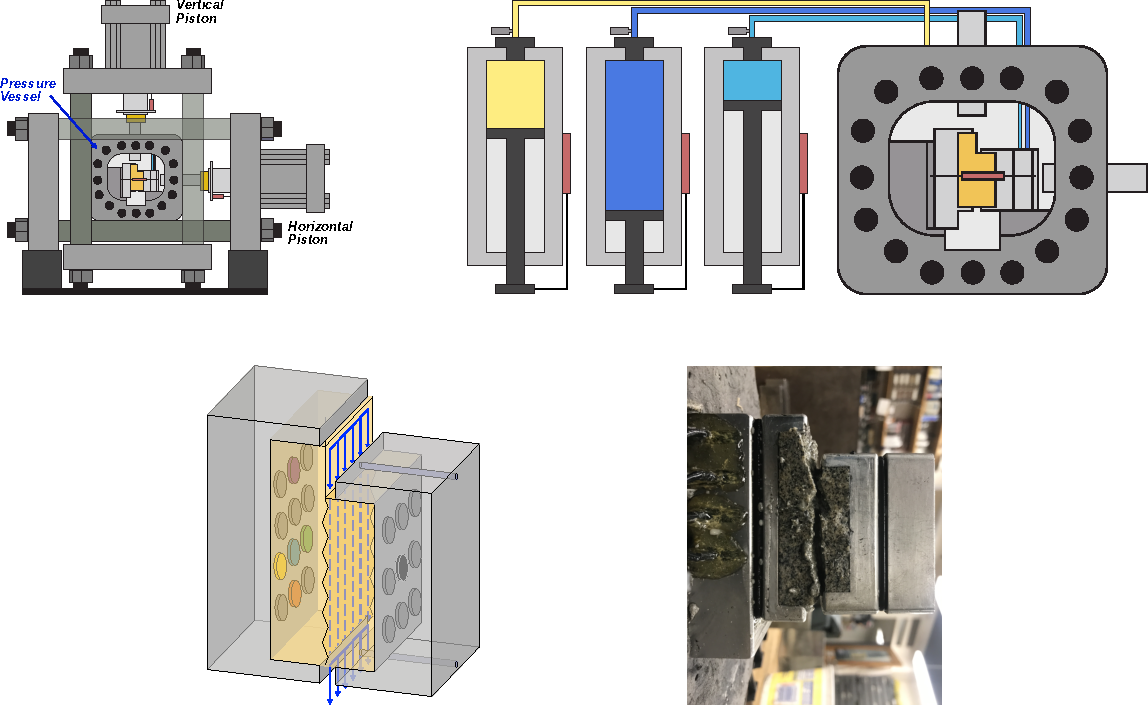
\includegraphics[width=0.9 \columnwidth]{exp_config.pdf}
	\caption[]{(a) The experiments were conducted in the Penn State Rock and Sediment Mechanics laboratory using the Biaxial Deformation Apparatus (Biax). The Biax has servo-controlled vertical and horizontal pistons and a 10 kHz 24-bit analog to digital data recorder. (b) A pressure vessel was inserted in the Biax and connected to the pressure intensifiers, which control the confining ($P_C$), and sample ($P_{PA}$ and $P_{PB}$ ) fluid pressures. (c) The Westerly granite sample is machine cut into a L-shape and placed between the two loading platens. These loading platens are embedded with piezoelectric transducers (p-polarized) and contain fluid ports for the inlet and outlet flow. The shorter forcing block additionally contains internal conduits to provide fluid flow along the fracture plane. Deionized water was pumped through these narrow channels (45 x 1 mm) and covered by sintered porous fits and fed by five 1.6 mm diameter holes. Sintered porous frits (permeability $\sim 10^{-14}\ m^2$) are press-fit into cavities within the short forcing block to allow homogeneous distribution of fluid. After securing this Single Direct Shear (SDS) configuration, it was sealed inside a latex jacket to separate confining and pore fluids. (d) A photo of the sample after experimentation highlights the degree of roughness of the in-situ fracture.}
	\label{fig:samplesetup} 
\end{figure*}

\newpage

\begin{figure*}[ht]
	\centering
	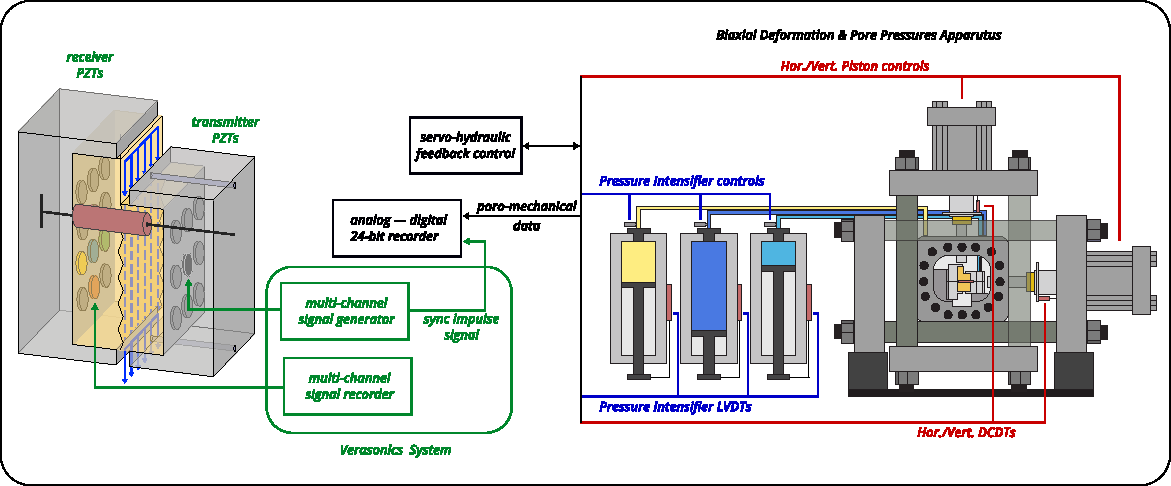
\includegraphics[width=0.9 \columnwidth]{exp_daq_v1}
	\caption[]{Schematic of the single direct shear configuration with the block diagram showing the main features of the data acquisition system for both the poro-mechanical and ultrasonic data. The Biax consists of two hydraulic pistons capable of applying vertical and horizontal loads in displacement or load control. Forces are measured using custom-built, beryllium-copper strain-gauge load cells mounted on each loading piston. The load cells have an amplified output of 5 V with an accuracy of 5 N and are calibrated with a Morehouse proving-ring. Displacements are measured with direct-current displacement transducers (DCDT), with an accuracy of $\pm 0.1 \mu m$. Each axis of loading is independently servo-controlled and all stresses, strains, fluid pressures and fluid volumes were recorded with 10 V, 16-channel 24-bit analog-to-digital converter at 10 kHz and averaged to sampling rates of 100 Hz or 1 kHz. Fracture permeability was measured using upstream and downstream pore-pressure intensifiers. Active ultrasonic data were recorded using a Vantage TM Research Ultrasound (Verasonics) system. We use broadband (0.02-2 MHz) PZTs (APC International Ltd. 6.35 mm diameter compressional crystals), which were successively pulsed every 1 ms on the transmitting side and the recording rate at the receiver side was 25 MHz. The input signal is a half sine with a frequency of 500 kHz. Also, a pulse from the Verasonics system accompanied the PZT excitation and is recorded by the 24-bit analog-to-digital data acquisition system. This allows us to sync the ultrasonic to poro-mechanical data and then analyzed to measure changes in the permeability and elasticity of the fractured rock samples, explained more fully in the signal analysis procedure.}
	\label{fig:data_aq}
\end{figure*}

\newpage

\subsection{Dynamic Effective Stress Perturbations}
The fractured samples were dynamically perturbed via pore pressure ($P_P$) and normal stress ($\sigma_{n}$) oscillations. Following the procedure described by Candela et al., 2015, pore pressure oscillations were achieved by oscillating $P_{PA}$ while holding $P_{PB}$ constant. Conversely, normal stress oscillations were
applied by oscillating the horizontal piston of the load frame at prescribed amplitude and frequency. 
As depicted in Figure 2a, multiple sets of Pp and $\sigma_n$ oscillations of varying amplitude (up to about $\pm$ MPa) and frequency (0.1, 1, 10 and 40 Hz) were applied to investigate the repeatability as well as amplitude and frequency dependencies of the measured response. Similar parameters were used for $P_P$ and $\sigma_{n}$ oscillation sets in order to apply similar effective stress perturbations and allow making comparisons between $P_P$ and $\sigma_{n}$ stimulations.


\subsection{Permeability Measurements}
\paragraph{} We measured flow rates independently at the inlet ($Q_A$) and outlet ($Q_B$) using the outputs of LVDTs on the pressure intensifiers. After verifying the steady state flow condition ($Q_{A} - Q_{B}  \leq 5 \% $), Darcy’s law was
used to calculate permeability k: 
\begin{equation} \label{eq:perm}
k = \frac{\mu L}{S} \frac{Q}{\Delta P_P}
\end{equation}
where $Q = \frac{1}{2} (Q_A + Q_B )$ is the average flow rate ($\frac{m^3}{s}$), $\mu$ is the fluid viscosity ($10^{-3} Pa\cdot s$) at 20\textdegree\ C, $L$ is the flow path given by the length of the sample (50 mm) and $S$ is the cross section perpendicular to the flow path (45 x 26 $mm^2$).
\paragraph{} Specifically, k is the bulk permeability, that is, the permeability of the surrounding rock matrix (on order of $10^{-21} m^2$) and of the fracture [Zhang et al., 2017; Ishibashi et al., 2018]. Alternative calculations of permeability are valid [Zhang et al., 2017; Ishibashi et al., 2018], however we are interested in relative changes in permeability in response to dynamic stressing, so the absolute value of the permeability is not necessary to quantify.


\subsection{Ultrasonic Measurements: Active Source}
Ultrasonic waves transmitted through the fracture were recorded continuously in each experiment. Half-cycle sinusoidal pulses with an amplitude of 40 V and center frequency of 500 kHz were emitted consecutively from each transmitting transducer (9 piezoelectric discs arranged in a 3 x 3 matrix embedded within the right-hand loading block in Figure 1b) with a pulse repetition frequency (PRF) of 100 Hz or 1000 Hz during the low and high frequency ($\geq 10$ Hz) stress oscillations, respectively. The waveforms were amplified ($\sim 40$ dB) and recorded for all the receiving transducers (12 piezoelectric discs arranged in a 4 x 3 matrix embedded within the left-hand loading block in Figure 1b). We activated up to the full array of 9 transmitter and 12 receivers. 

\newpage

\begin{figure*}[ht]
	\centering
	%	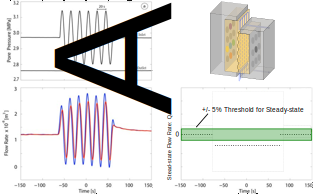
\includegraphics[width=1.0\columnwidth]{PpFlow_fig_v1}
	%	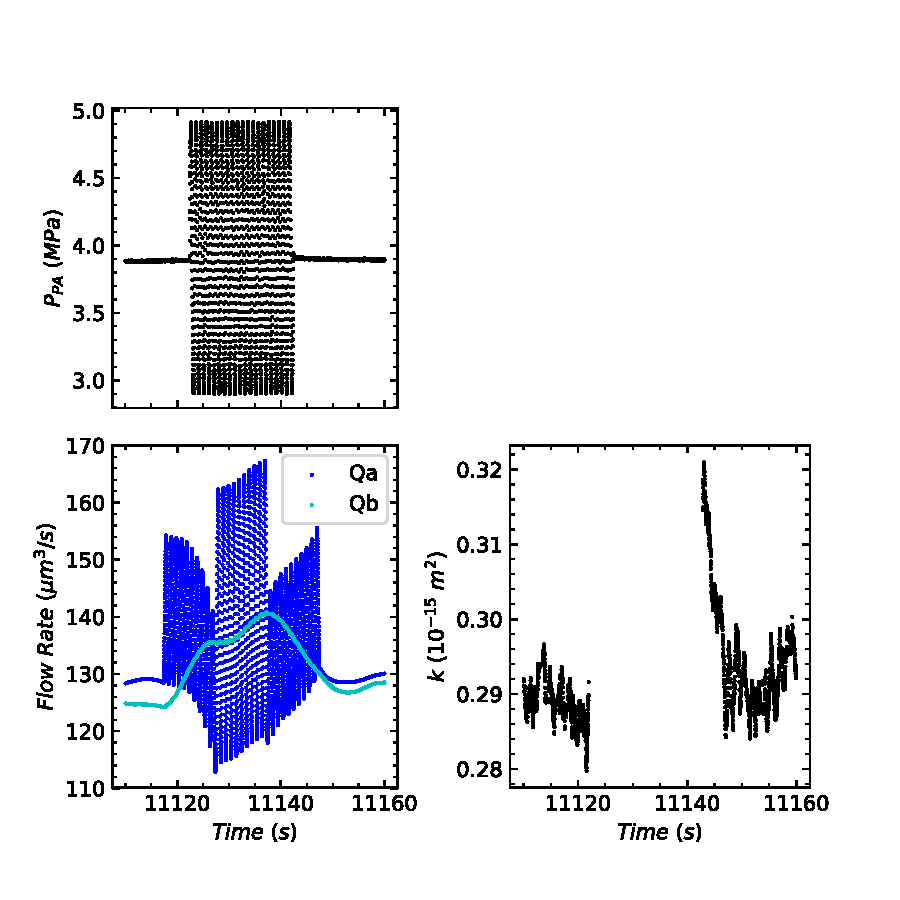
\includegraphics[width=0.8\columnwidth]{permCalcPlots_p4975_run3b_1Hz}
	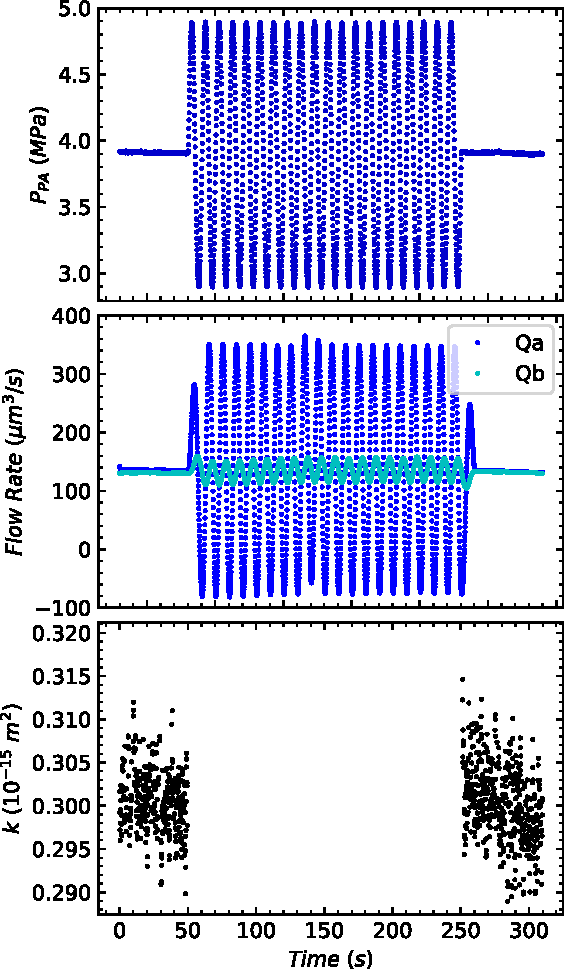
\includegraphics[width=0.4\columnwidth]{permCalcPlots_tall_p4975_run3b_1Hz}
	\caption[]{Example of dynamic stressing and the corresponding flow rate measurements for a set of pore pressure oscillations in experiment p4975. Note that the plots (a) and (b) are decimated for clarity. (a) Imposed pore pressure oscillation at inlet and fixed pore pressure at the outlet. Pressure conditions before and after the oscillations are identical. (b) Measured flow rates at the fracture inlet (blue line) and outlet (red dashed line). Notice the small time lag ($\leq$ 2 s) between the maxima of the inlet and outlet flow rates. (c) Permeability at steady-state and during the pore pressure oscillation. In the calculation of permeability we impose a threshold between the flow rates to ensure steady-state flow ($Q_{A} - Q_{B}  \leq 5 \% $). It is reasonable to assume that even at relatively low frequency oscillations, there is effectively no steady-state flow during the imposed oscillations.}
	\label{fig:exp_over}
\end{figure*}

\textcolor{red}{We measure the effective permeability, ka, by calculating the flow rate over a 2 s window. For pore pressure oscillations, we start 10 s after the oscillation to ensure that permeability measurement is not affected by the Pp oscillation and/or by storage effects. Need to annotate Flow Rate with lines indicating the +- 5\%}

\newpage

\begin{figure*}[ht]
	\centering
	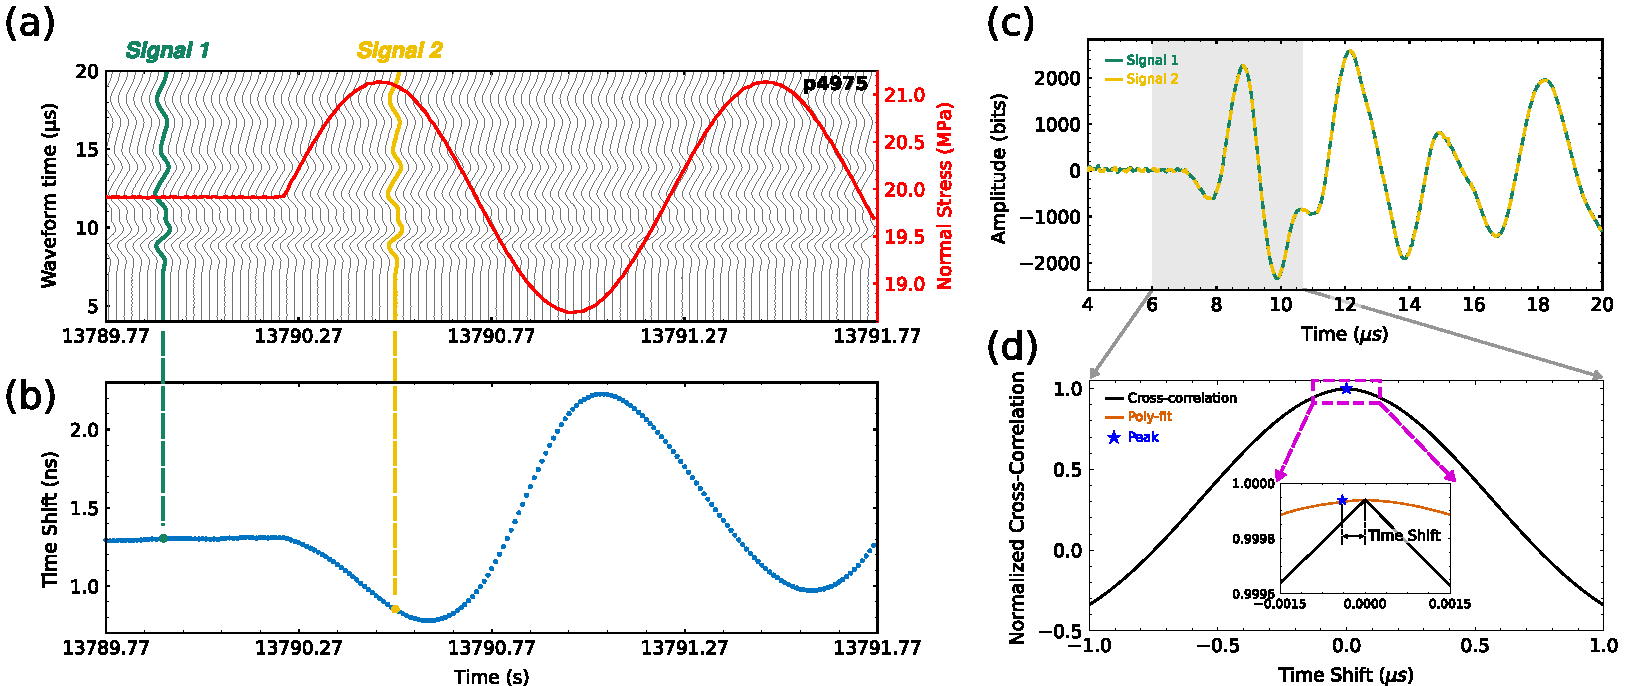
\includegraphics[width=0.9 \columnwidth]{xcor_fig_v3}
	\caption[]{(a) Excerpt from run4 of experiment p4966 shows part of a 1 Hz, 1 MPa normal stress oscillation (red) and the concurrent raw ultrasonic waveforms (grey). The number of waveforms in the waterfall plot has been decimated version for clarity. (b) Time shift was calculated by cross-correlating the waveforms to a reference waveform. (c) An example of a reference, unperturbed, waveform (green) and perturbed waveform (dashed yellow) highlights
		the similarity. (d) The maximum linear correlation between the reference and perturbed waveforms from cross-correlation is used to determine the time shift. The inset shows improvement of time shift calculations with a 2nd order polynomial fitting procedure.}
	\label{fig:xcor_poly}
\end{figure*}

\newpage


\section{Experimental Procedure}

\begin{figure*}[ht]
	\centering
	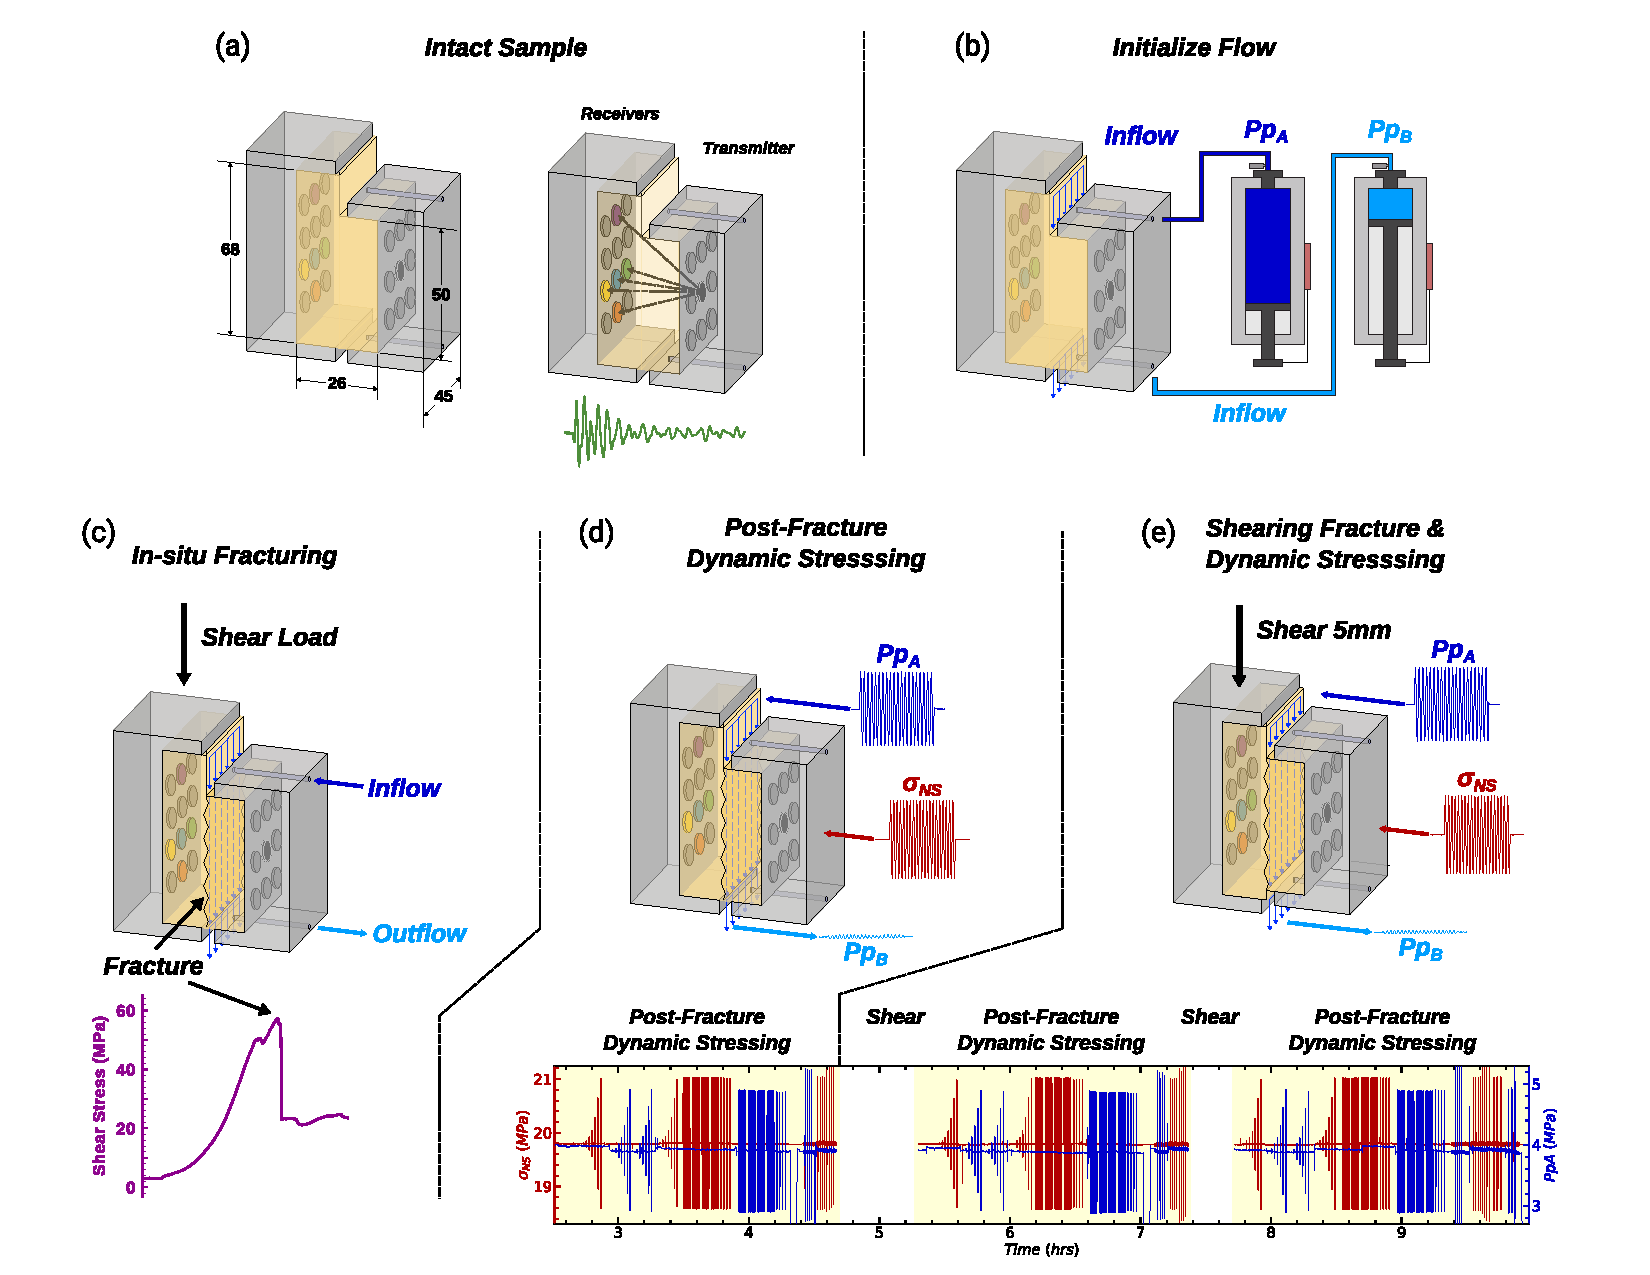
\includegraphics[width=1\columnwidth]{exp_sequence}
	\caption[]{We conducted sophisticated experiments in which samples were loaded under triaxial conditions inside a pressure vessel and fractured in-situ to simultaneous measure flow rate and elastic properties. (a) Westerly granite samples were prepared by cutting them into L-shape blocks (68 x 45 x 50 x 26 mm), with 3 mm deep notches on the top and bottom to ensure reproducibility of planar fracture propagation. The L-shape is used for maintaining constant nominal contact area during fracture and shear. The samples were saturated in deionized water and then placed between steel forcing blocks that have embedded piezoelectric transducers. The spacing between the steel loading platen and the PZTs is 4mm. The approximate ray paths from the transmitter to receivers are illustrated in the right part of this panel. A sample waveform, consisting of compressional, shear, and coda components, is shown below in green.
	}
	\label{fig:exp_seq}
\end{figure*}

\newpage

...Continued from Figure \ref{fig:exp_seq}...

(b) Next, we applied a pore pressure differential: inlet ($P_{PA}$ = 4 MPa) and outlet ($P_{PB}$ = 2 MPa). At this point there was no flow because Westerly granite matrix permeability is very low ($< 10^{-20}\ m^2$ ) and the confining fluid pressure is greater than the pore pressure (preventing flow of water around the sample).
c) The sample was then fractured in situ by increasing the shear stress at constant normal stress while making continuous measurements of fluid flow and ultrasonic properties. The loading curve is illustrated below, the critical shear stress was $ \approx $60 MPa. 
(d) After locking the vertical piston (constant displacement), we executed the dynamic stressing protocol. Pore pressure oscillations were achieved by oscillating $P_{PA}$ while holding $P_{PB}$ constant. Normal stress oscillations were applied by oscillating the horizontal piston of the load frame at prescribed amplitude and frequency. Multiple sets of $P_{P}$ and $ \sigma_{NS} $ oscillations of varying amplitude (up to about $ \pm $ 1 MPa) and frequency (0.1, 1, 10 and 40 Hz) were applied to investigate the repeatability as well as amplitude and frequency dependencies of the measured response. Similar parameters were used for $P_{P}$ and $ \sigma_{NS} $ oscillation sets in order to apply similar effective stress perturbations and allow making comparisons between $P_{P}$ and $ \sigma_{NS} $ stimulations, as seen in excerpt plot below. Post-fracture dynamic stressing is highlighted with a yellow box. 
(e) To investigate the effect of fracture aperture on elastic nonlinearity and permeability, the sample was sheared 5 mm, held at $ \sigma_{NS} $ = 20 MPa. Initially,the in-situ fracture was quite rough, but the effect of shear reduces and changes this roughness (shear changes the number of fracture asperities in contact and extent to which the two halves were mated) and thus allows for investigation of how fracture aperture is related to the elasto-dyamic and hydromechanical properties. The plot below shows the dynamic stressing and shear sequence imposed on the sample.

\newpage




\paragraph{}
We measure the nolinearity of the elastodynamic response directly by quantifying the stress-dependency of wave velocity and amplitude. Figure X depicts the typical response of our fractured samples to dynamic stress perturbations. Immediately after effective stress oscillations, the fractured rock exhibits an instantaneous softening i.e., the wave velocity $c_0$ suddenly drops. However, if the dynamic perturbation is not too strong, this softening is transient; once the oscillation is removed, the wave velocity oscillates in response to dynamic stress at frequencies hat are harmonics of the excitation frequency. The averge amplitude of these oscillations (at the oscillation frequency) is denoted as $dc$ in Figure X. If the stress oscillations persist, the changes in wave velocity reach a non-equilibrium steady state. This characteristic response (transient softening, slow recovery and velocity fluctuations) is a signature of nonlinear mesoscopic elasticity (Guyer and Johnson, 2009) and rich in information on microstructure, fractures and contact mechanics. In comparison, the wave velocity in a linear elastic medium is stress-invariant i.e., $c = c_0$ before, during and after stress oscillations. Most intact rocks exhibit some degree of nonlinearity due to soft grain boundaries and microcracks in their matrix (Rivière et al., 2015). However, when fractured, their nonlinear electrodynamic responses are also influenced by the contact acoustic nonlinearity (CAN) at the rough fractured interface.  

\paragraph{}
In order to quantify the nonlinearity of the fractures, we first obtain the evolution of ultrasonic wave amplitude (Figure 2b) and velocity (Figure 2c) from the continuously measured ultrasonic data  (Shokouhi et al., 2019) and calculate three parameters: (1) the average or DC-change in wave velocity due to the imposed oscillations, (2) the amplitude of steady-state velocity fluctuation during the oscillations, and (3) the recovery rate of wave velocity post oscillation (Figure 2c). The relative velocity change ($\Delta c/c_0$)
is defined as the \% change in velocity due to the imposed normal stress or pore pressure oscillation. We calculate $\Delta c/c_0$ 
from the velocity before ($c_0$) and after ($c$) each oscillation averaged over 1-s time windows as depicted in Figure 2c. At a given oscillation amplitude, the more negative the $\Delta c/c_0$ (larger absolute value), the more nonlinear is the fracture. The parameter 
$dc/c_0$ is defined as the amplitude of velocity oscillations, averaged over the oscillation duration and normalized by pre-oscillation velocity $c_0$ (Figure X). Similar to $\Delta c/c_0$, a larger magnitude of $dc/c_0$ at a given oscillation amplitude is an indication of higher nonlinearity. The third parameter 
$\dot c$.
is defined as the (logarithmic) rate of recovery of wave velocity after the oscillation is removed (Figure 2c). Materials of higher nonlinearity are expected to have slower recoveries (Shokouhi et al., 2017b). In the next section, we discuss the dependence of 
$\Delta c/c_0$, $dc/c_0$, and $\dot c$ 
(Figure X) on the imposed normal stress and pore pressure amplitudes as well as frequency.  In addition, we compare the measured nonlinearities before and after shearing the fracture. This comparison provides insight into how changes in the aperture size distribution (due to shearing and wear) and the presence of fines alter the fracture stiffness and the stress-dependency of the elastodynamic response. Although not shown here, similar nonlinearity parameters may be extracted from the evolution of ultrasonic wave amplitude (Figure X). 


\newpage

\begin{figure*}[ht]
	\centering
	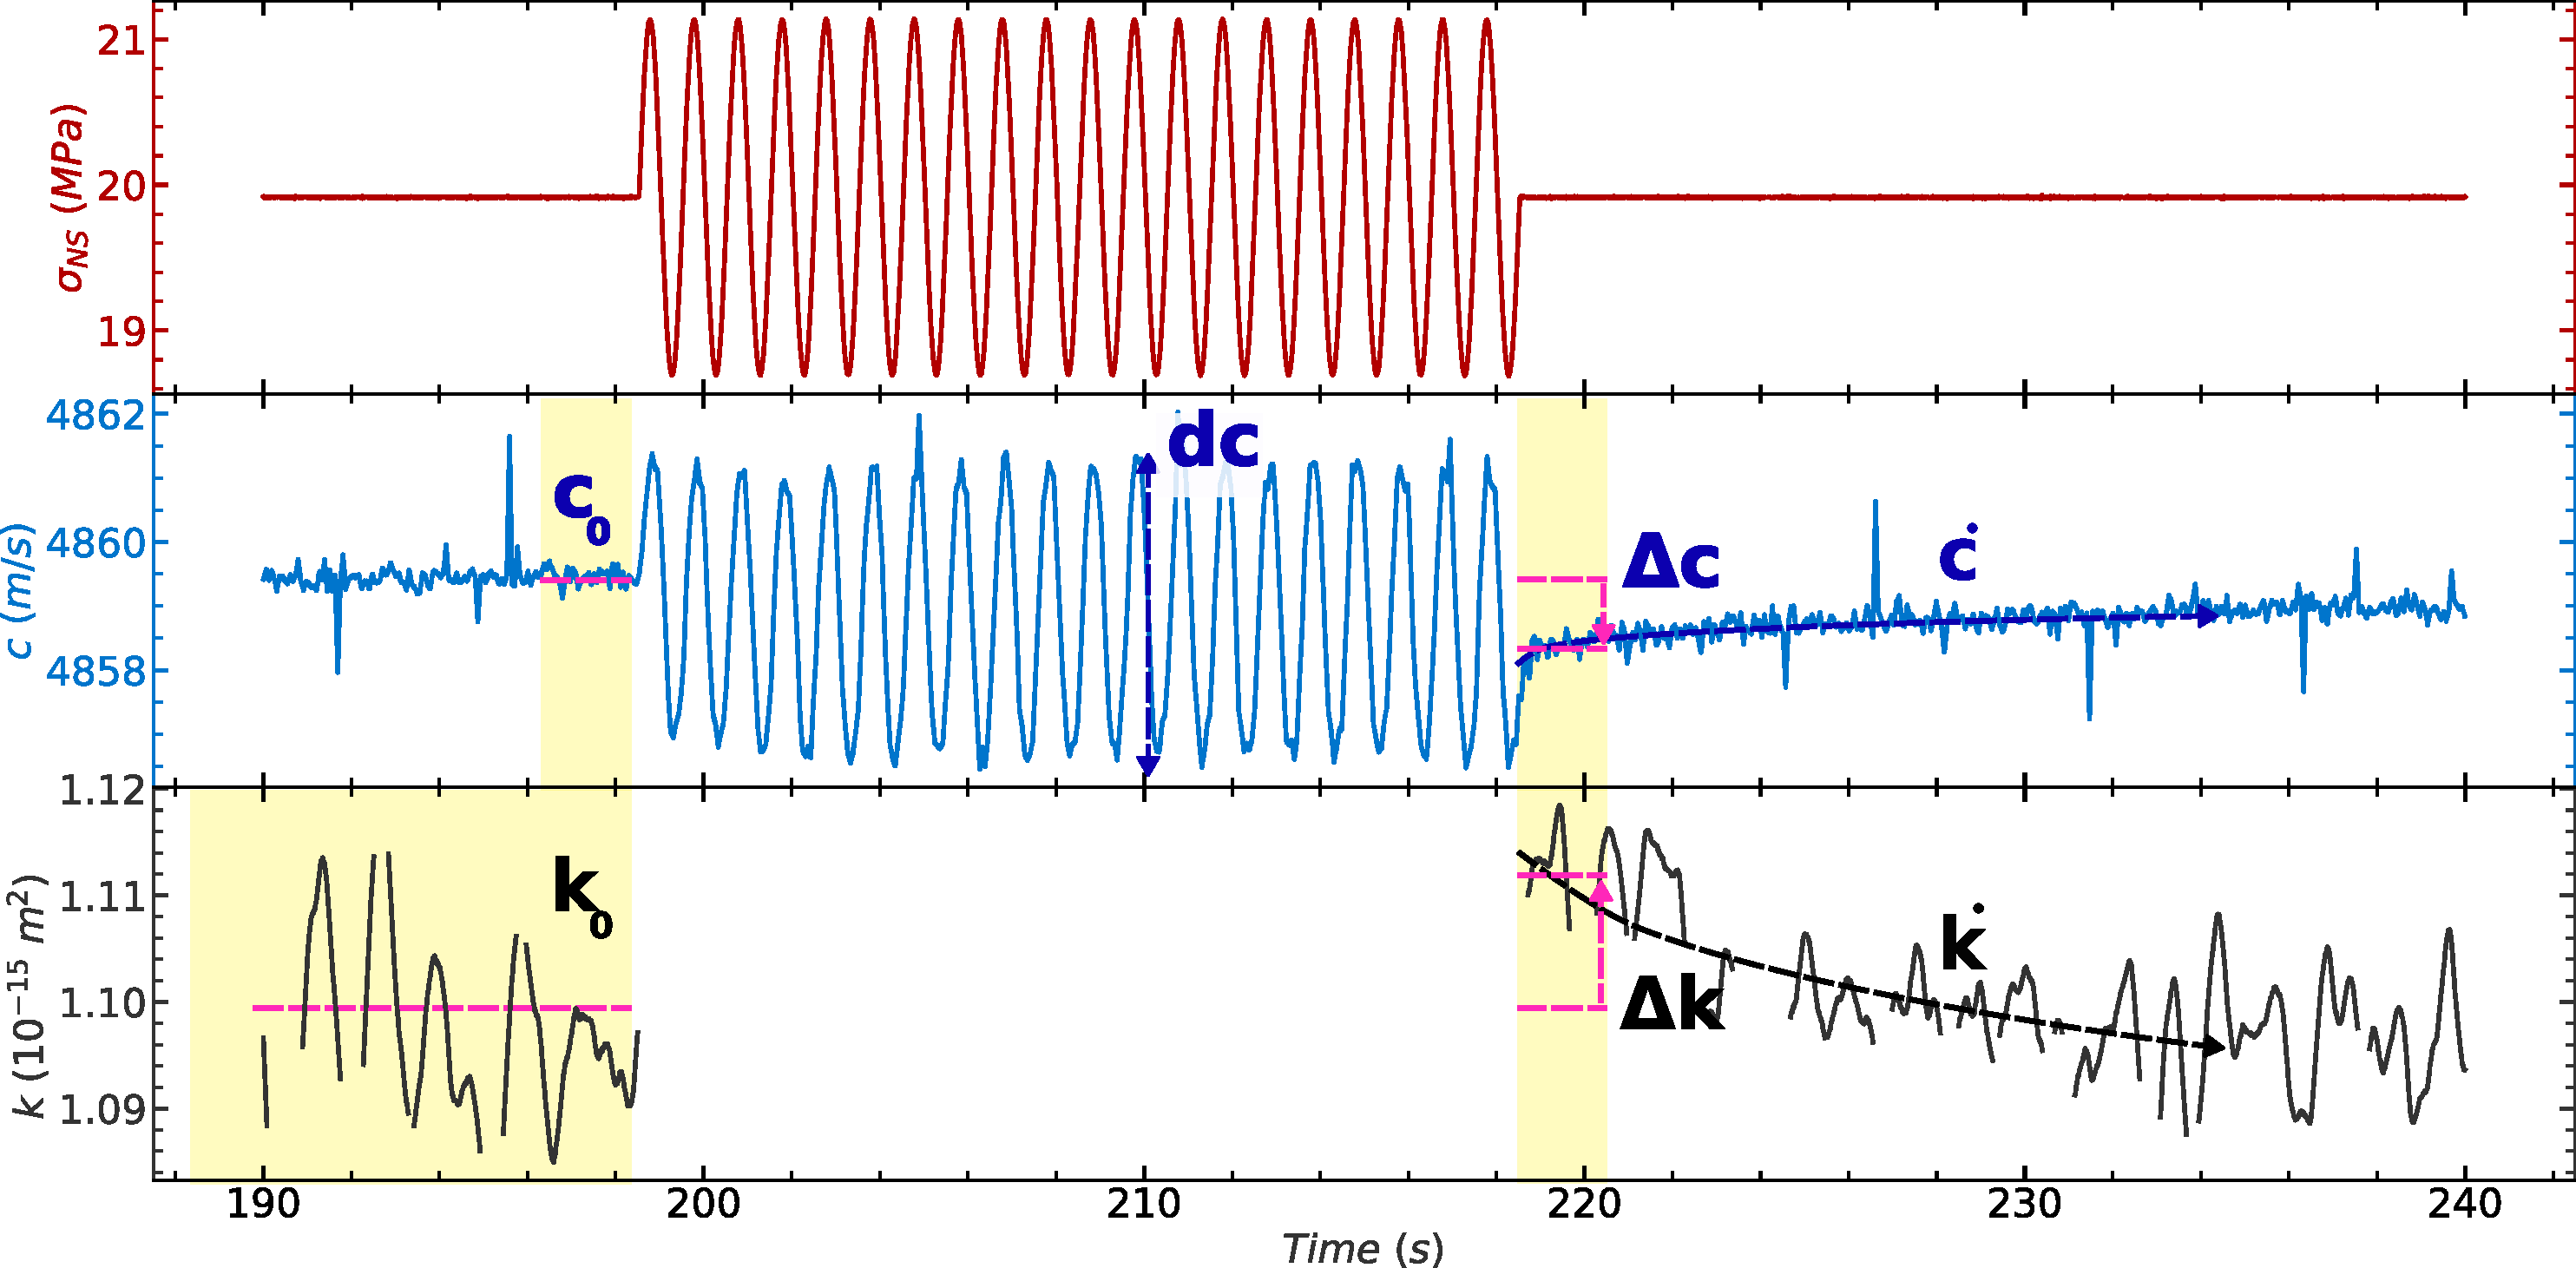
\includegraphics[width=0.9\columnwidth]{NsPpaKexp_edit}
	\caption[]{The velocity and permeability changes are calculated using the measured values before and after each oscillation averaged over the time windows (gray boxes) shown in (c). Data points in the permeability measurements are omitted on the condition that inlet/outlet flow rates differ $ > 5 \% $. That is to say, plotted permeability points represent when there is steady-state flow, necessary for Darcy’s law. Dashed lines indicate the recovery of p-wave velocity ($ \dot c$) and permeability ($\dot k$), respectively, from post-oscillation response to new steady-state value. Furthermore, we parameterize the p-wave velocity change dc during the normal stress or pore pressure oscillations, indicated by dashed blue line.}
	\label{fig:delc_delk_calc}
\end{figure*}

\newpage

\begin{figure*}[h]
	\centering
%	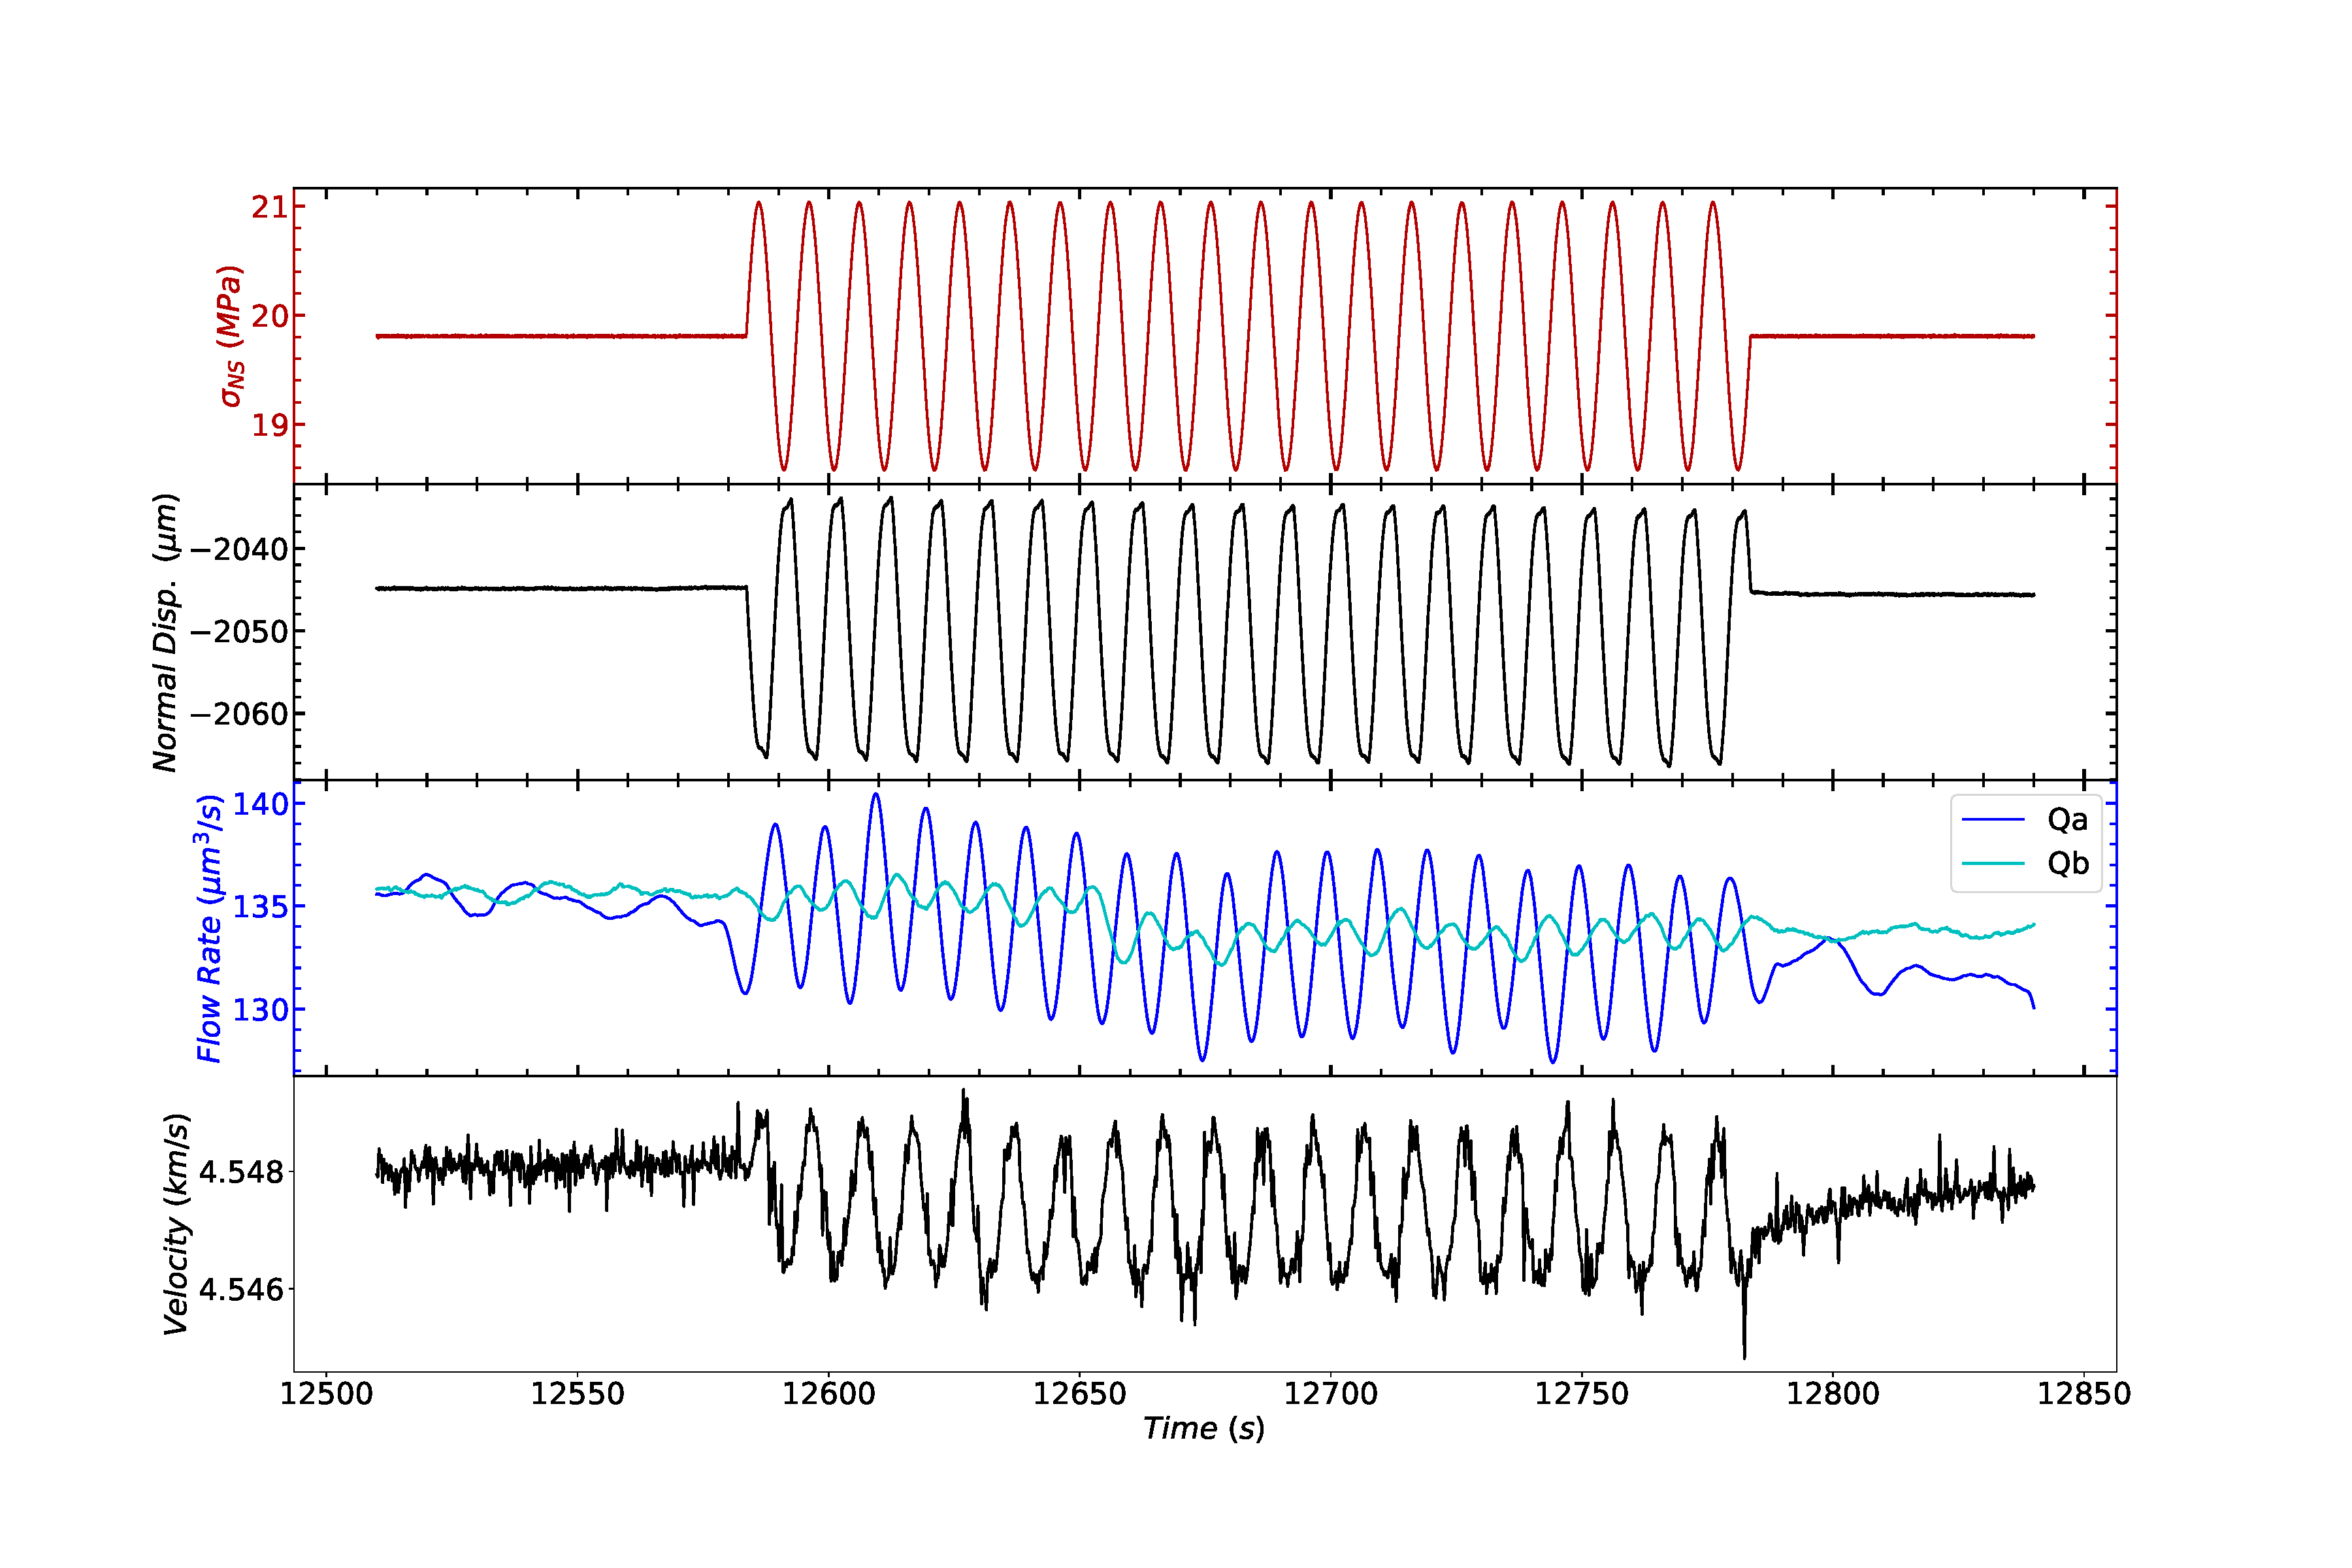
\includegraphics[width=0.8\columnwidth]{NS_p4975_run3b_01Hz}
%	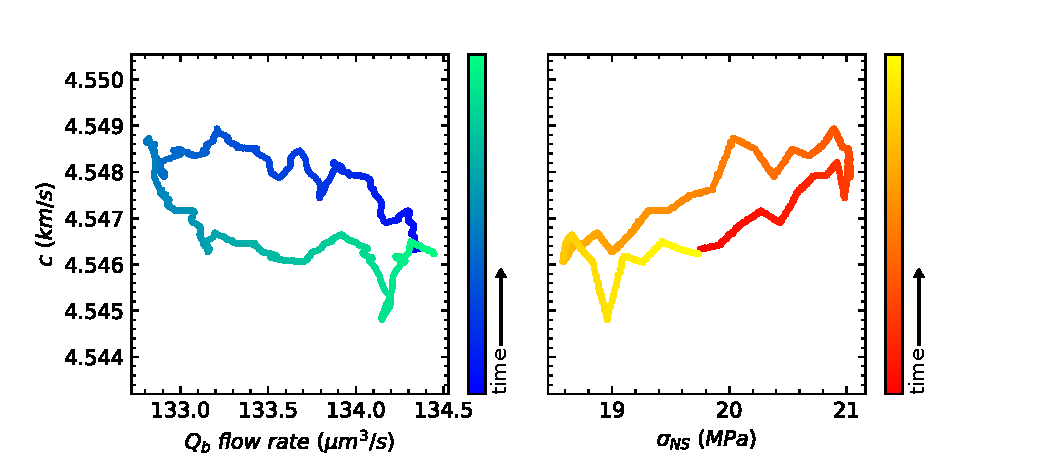
\includegraphics[width=0.7\columnwidth]{NSbowtie_p4975_run3b_01Hz_Cycle19}
	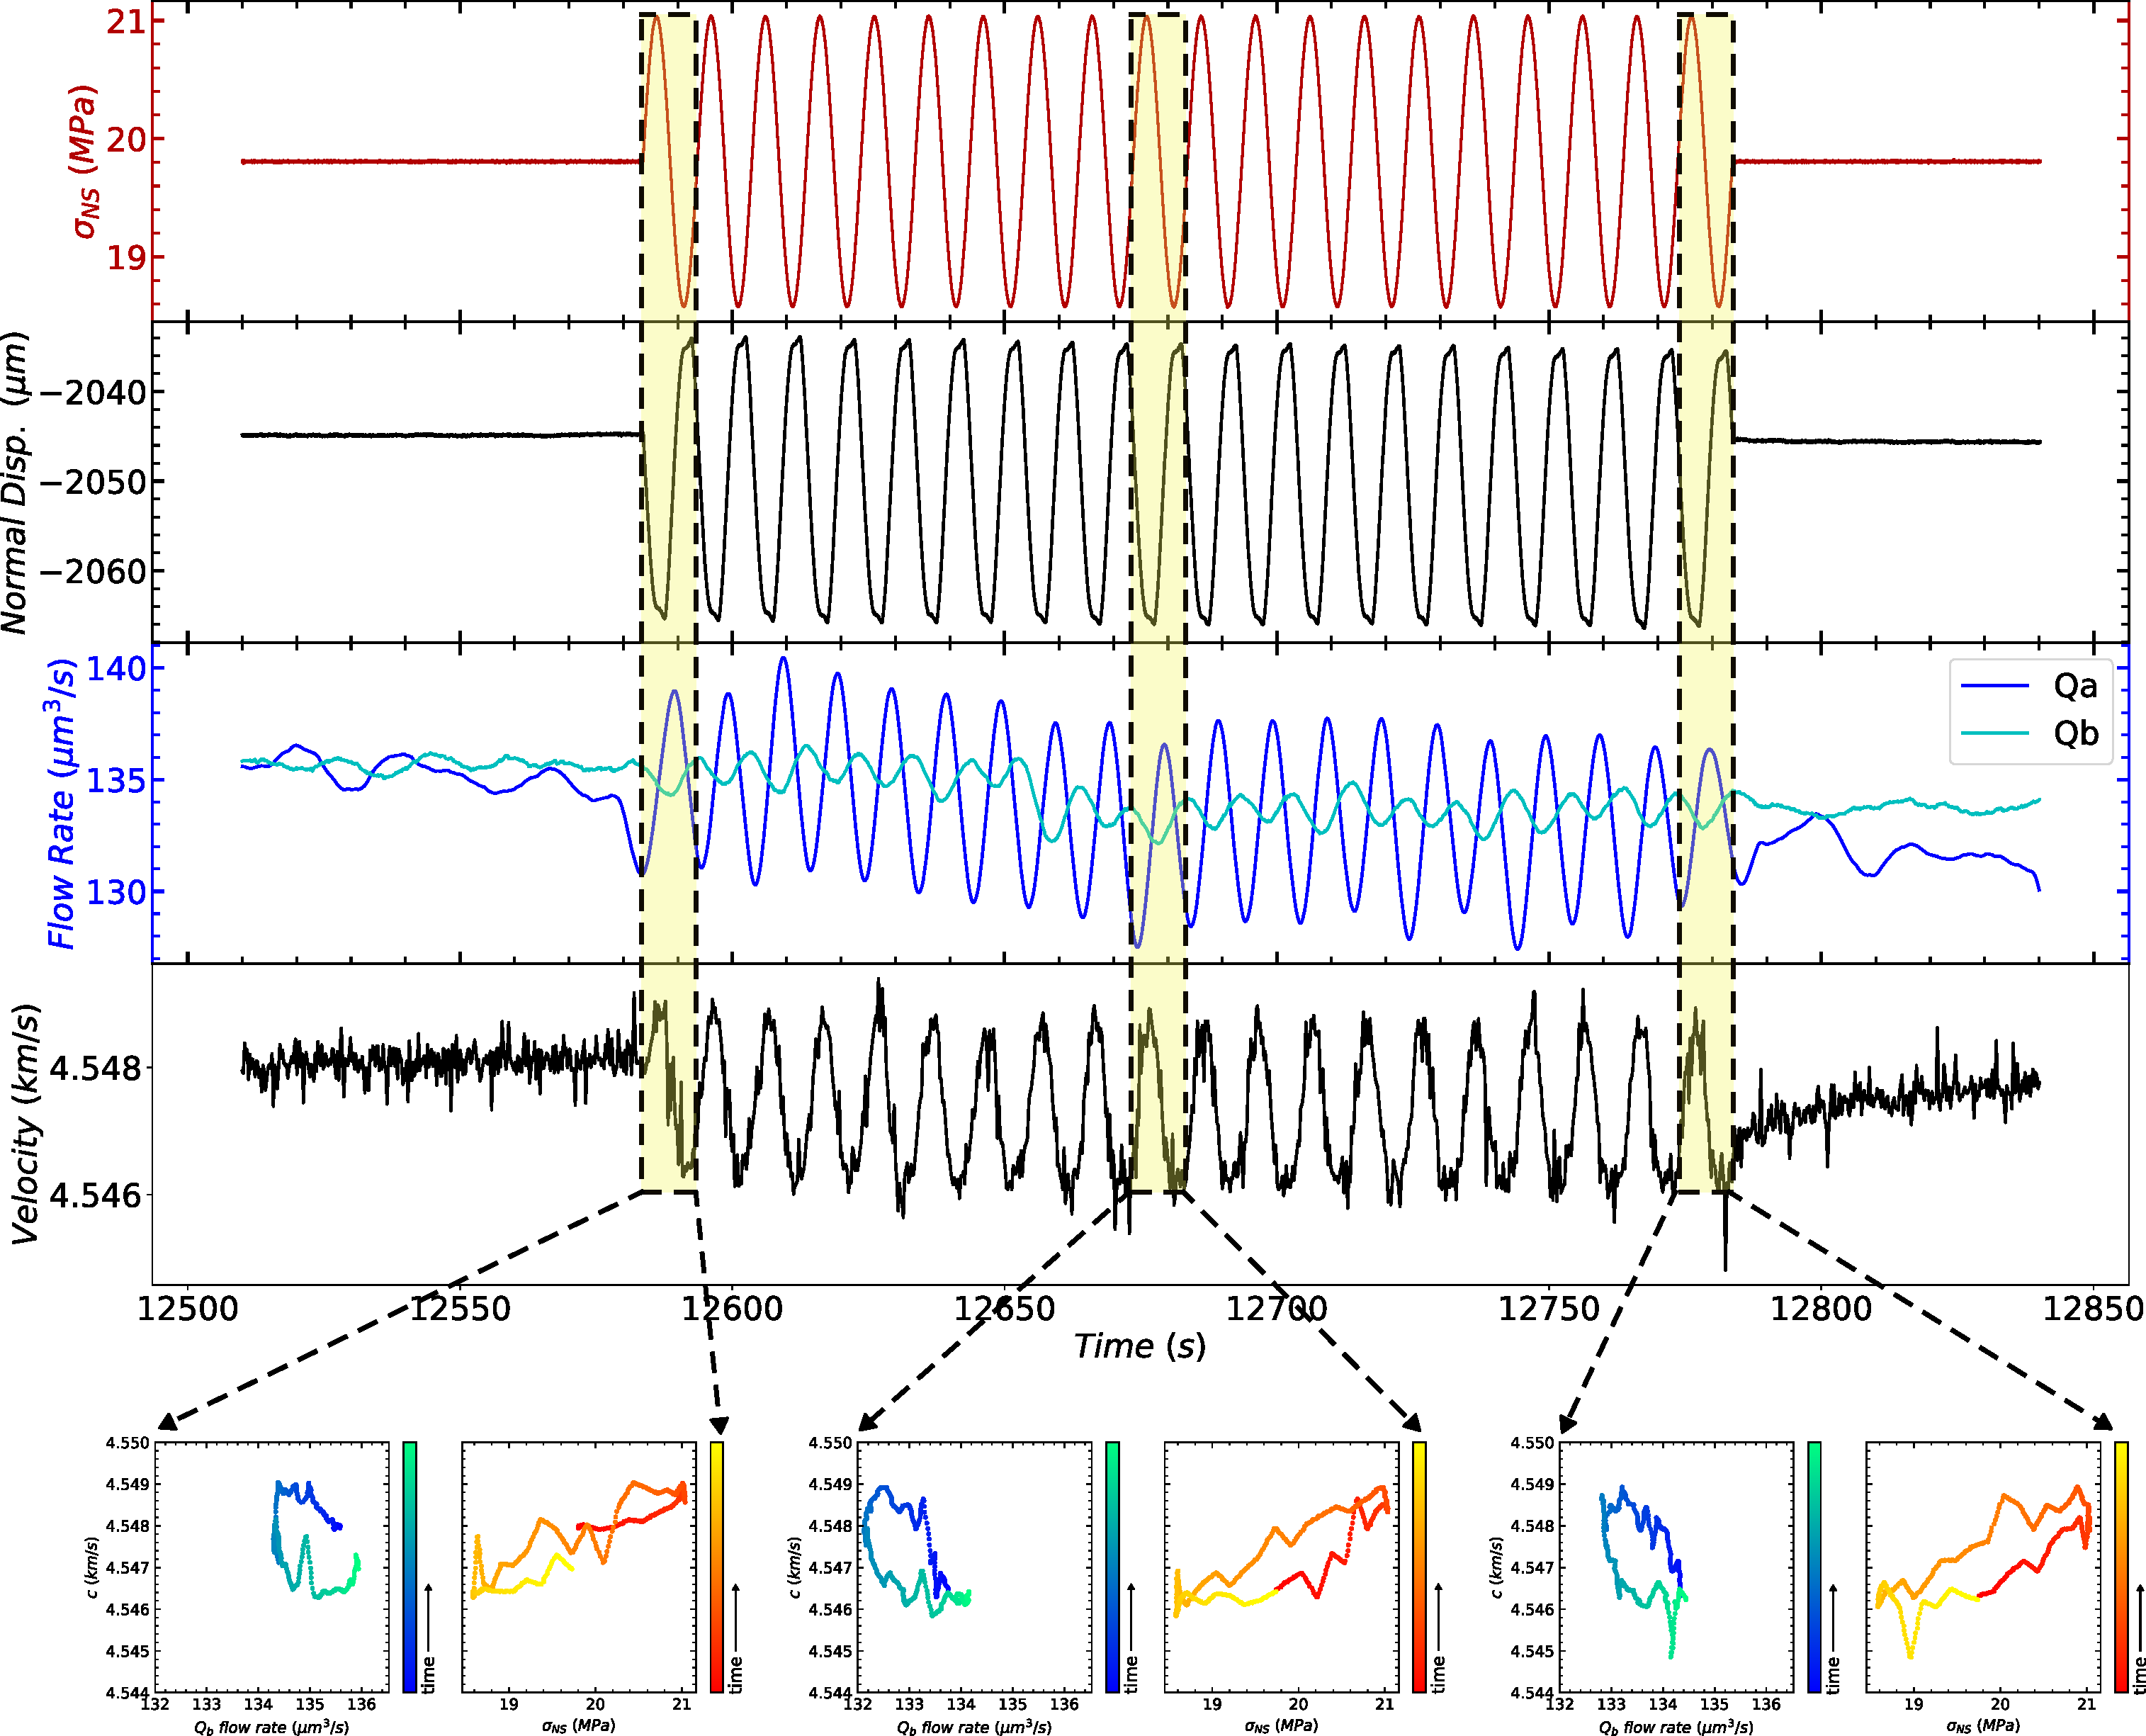
\includegraphics[width=0.99\columnwidth]{NS_bowtie_p4975_run3b_01Hz}
	\caption[]{(a) Direct response of normal displacement, flow rate (inlet and outlet), and ultrasonic velocity for the direct path pair during a 0.1Hz 1MPa Normal Stress oscillation. Note the phase delay between the inlet and outlet flow rates. (b) shows how velocity varies as a function of outlet flow rate, Qb, during the last cycle of the normal stress oscillation. The velocity increases with decreasing flow rate during compression and then the opposite trend with tension. The point to make here is that the fracture is continuously changing -- the change in aperture results in change in velocity and flow paths. (c) Ultrasonic velocity as a function of the last full cycle of the normal stress oscillation.}
	\label{fig:NS_p4975_run3b_01Hz}
\end{figure*}

\textcolor{red}{Delineate (b) \& (c) to distinguish compression and tension of oscillation.\\}

\newpage



%We quantify these changes with the following:\\
%\begin{equation} \label{eq:delc}
%\frac{\Delta c}{c_0} = \frac{c(\langle t_1 \rangle) - c(\langle t_0 \rangle)}{c(\langle t_0 \rangle)}
%\end{equation}
%\begin{equation} \label{eq:delk}
%\frac{\Delta k}{k_0} = \frac{k(\langle t_1 \rangle) - k(\langle t_0 \rangle)}{k(\langle t_0 \rangle)}
%\end{equation}
%We adapted the Akaike Information Criterion (AIC) into an algorithm to find the first arrival (cite paper here).
%\begin{equation} \label{eq:aic}
%AIC(k) = k \cdot \log(\sigma^{2}_{1,max}) + (N_{samp} - k -1) \cdot \log(\sigma^{2}_{2,max})
%\end{equation}


%\section{Discussion and Results: Permeability}
%
%\begin{figure}[ht]
%	\centering
%	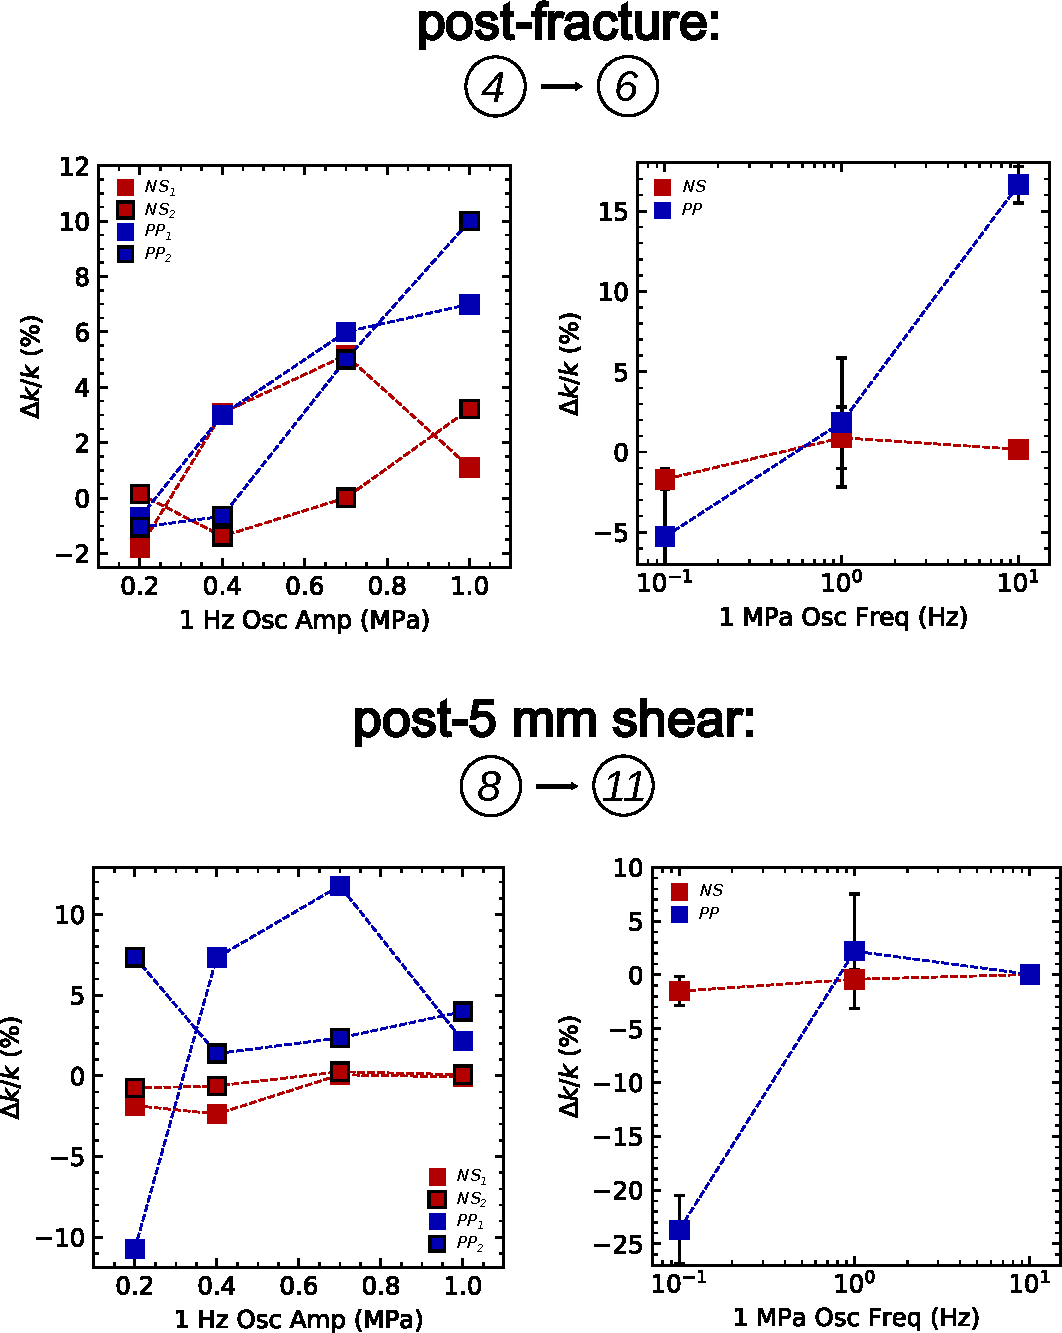
\includegraphics[width=6cm]{delperm}
%	\caption{The figure to the right shows the relative change in permeability as a function of amplitude (top row) and frequency (bottom row). In the post-fracture case, we see that pore pressure oscillations have a larger increase in permeability with increasing amplitude; we see a similar trend as well in the post-fracture runs.\\
%	Also, we report that there is a general increase in permeability as frequency of 1 MPa pore pressure oscillations increases for post-fracture runs. We see something less systematic for the post-shear runs. This is probably due to pore pressure oscillations mobilizing the fine grains at the interface, created by the initial fracture and then additional 5 mm of shear.}
%	\label{fig:delk_plots}%
%\end{figure}
%
%\pagebreak

\section{Results}
\subsection{Nonlinear Elastodynamic Response: Relative Change in Velocity and Permeability}
\begin{itemize}
	\item nonlinearity modulated by oscillation amplitudes
\item nonlinearity and permeability enhancement generally increase with frequency of dynamic stressing.
\item relative changes in wave velocity and permeabilityare correlated: larger drops in velocity —> larger increases in permeability
\item changes in permeability are greater at higher oscillation amplitudes 
\subitem Perm enhancement pronounced for Pp oscillations than for NS.
\end{itemize}


\begin{figure}[ht]
	\centering
	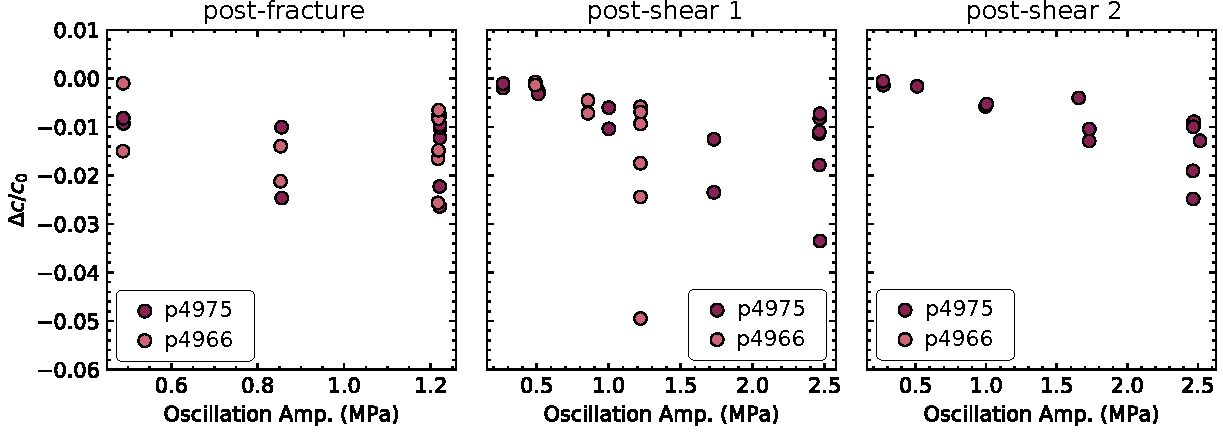
\includegraphics[width=0.9\columnwidth]{Delc_NS_amp}
	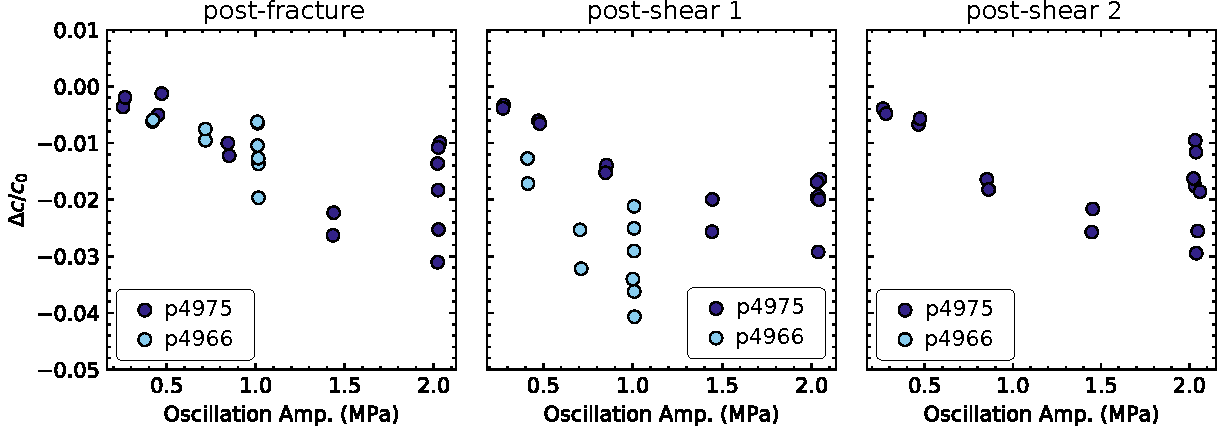
\includegraphics[width=0.9\columnwidth]{Delc_PP_amp}
	%\enspace
	%\includegraphics[width=6cm]{post-frac_amp_array}
	\caption{Nonlinearity as a function of $ \sigma_{NS} $ oscillation amplitude. Transitioning from post-fracture results to post-shear results, we observe decreased nonlinearity and permeability enhancement. This is probably related to clogging mechanisms.}%
	\label{fig:delc_ns_amp}
\end{figure}

\newpage

\begin{figure}[ht]
	\centering
	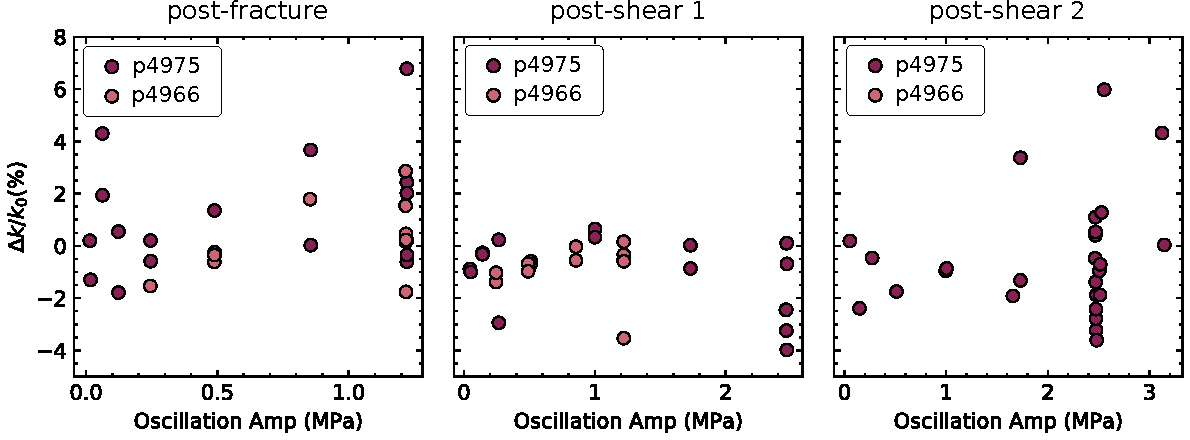
\includegraphics[width=0.9\columnwidth]{k_NS_amp}
	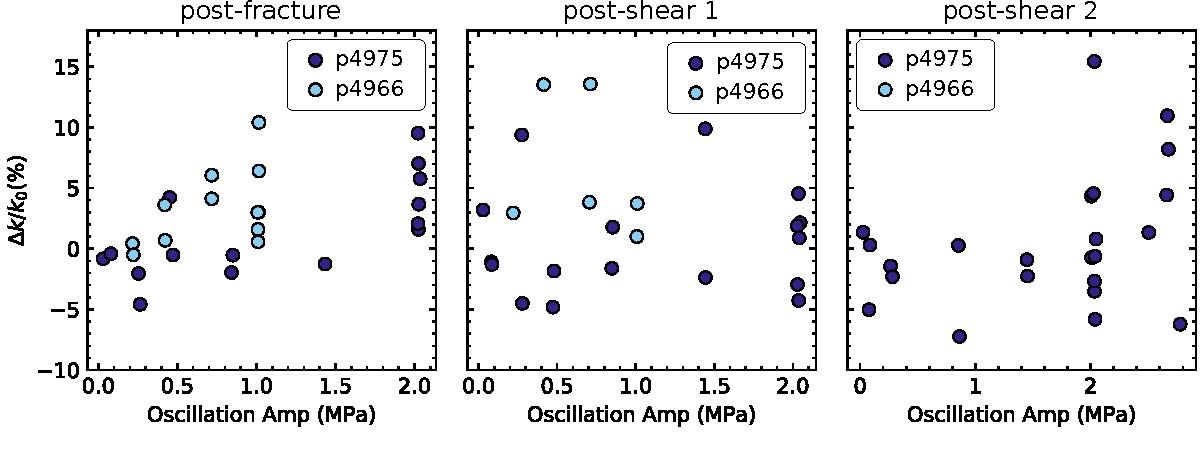
\includegraphics[width=0.9\columnwidth]{k_PP_amp}
	%\enspace
	%\includegraphics[width=6cm]{post-frac_amp_array}
	\caption{Change in permeability as a function of $ \sigma_{NS} $ oscillation amplitude. Transitioning from post-fracture results to post-shear results, we observe decreased nonlinearity and permeability enhancement. This is probably related to clogging mechanisms.}%
	\label{fig:perm_ns_amp}
\end{figure}

\newpage


\begin{figure}[ht]
	\centering
	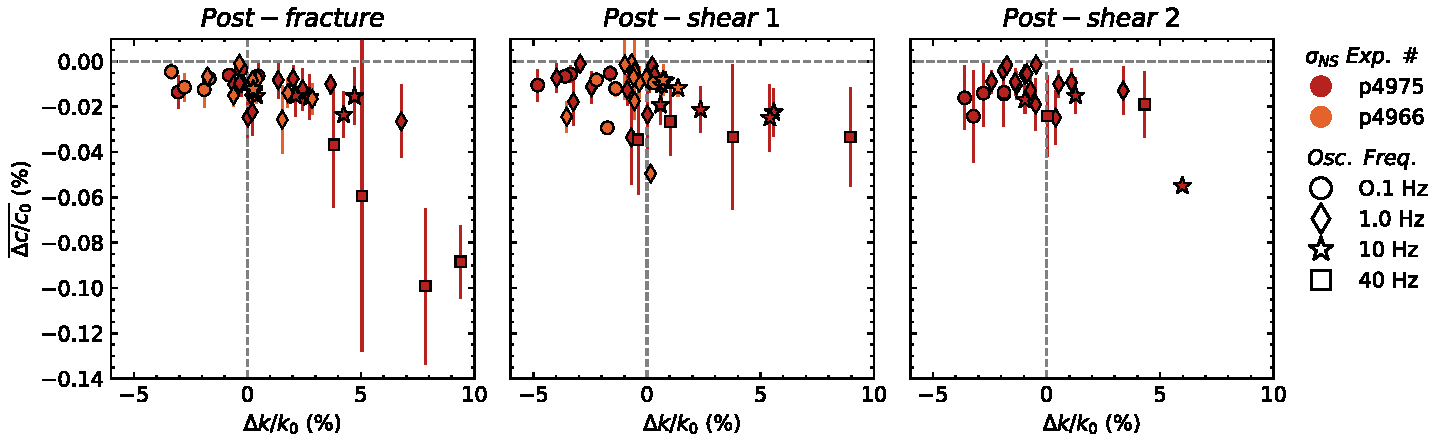
\includegraphics[width=1\columnwidth]{avgDelc_all_NS}
	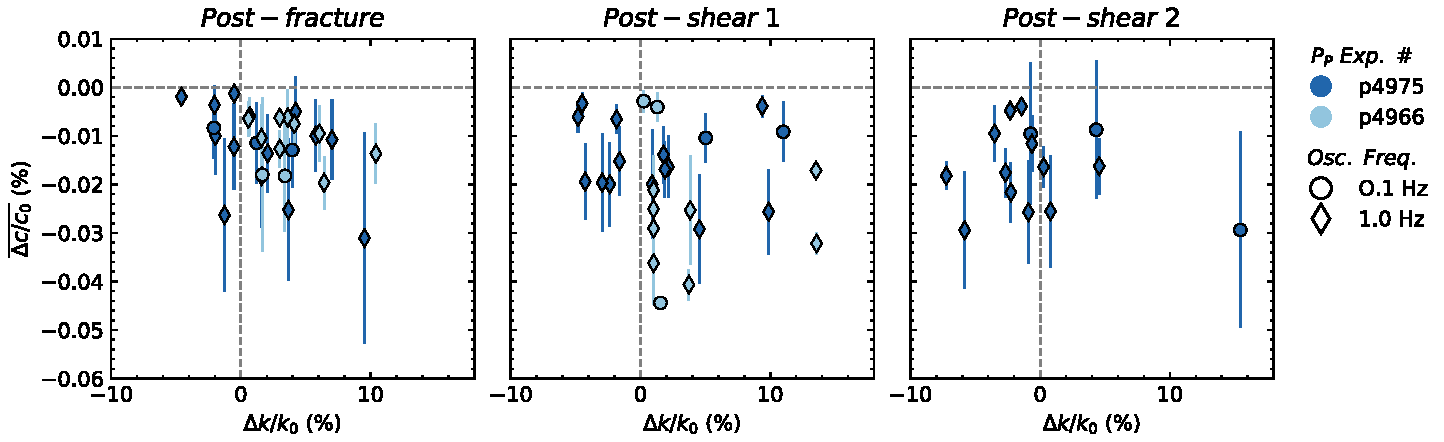
\includegraphics[width=1\columnwidth]{avgDelc_all_PP}
	%\enspace
	%\includegraphics[width=6cm]{post-frac_amp_array}
	\caption{Nonlinearity as a function of permeability change for $ \sigma_{NS} $ and $ P_P $ oscillations averaged over all receivers. Permeability is an averaged measurement across the fracture, so these parameters should exhibit some relationship. I don’t know what this says about the mechanisms at play. Maybe the contact area has been reduced (lower nonlin) and also maybe wear material was mobilized during Pp oscillation sand temporarily increased contact area (higher nonlin). Does this match with reality -- does shearing the fracture increase the contact area? My intuition agrees with this, but it is conceivable that with a complex geometry, this could be more complex.}
	\label{fig:delc_plots2}
\end{figure}

\newpage


\subsection{Velocity Amplitude Modulation during Perturbations}




\begin{itemize}
	\item Although the origins of $dc/c_0 $ and $ dc/c $ remain unclear, consider empirical evidence from [Rivière et al., 2015, 2016] that they originate from different micro-scale mechanisms 
\end{itemize}


\begin{figure}[ht]
	\centering
	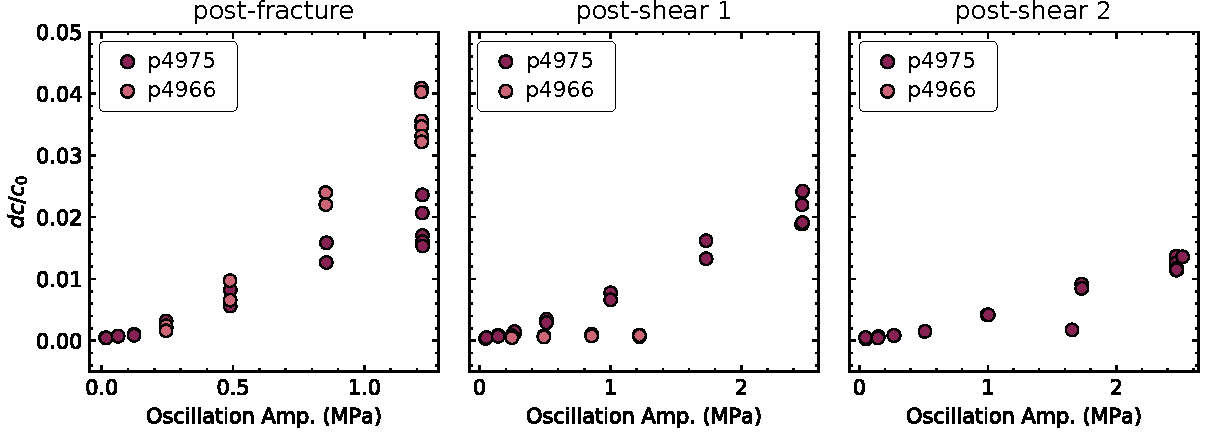
\includegraphics[width=1\columnwidth]{Dc_NS_amp}
	\includegraphics[width=1\columnwidth]{Dc_PP_amp}
	%\enspace
	%\includegraphics[width=6cm]{post-frac_amp_array}
	\caption{Velocity amplitude modulation averaged over all receivers ($ dc/c_0 $) as a function of permeability recovery ($ \dot k $) for NS and PP oscillations. 
		I suspect that the we are not waiting long enough to see a trend like J. Elkhoury and others. His recovery values were ~0.5, which he says is related to the dimensionality of the fracture. Shearing the fracture increases the complexity and maybe changes the slope -- dominated by clogging/moving wear material rather than mated aperture.}
	\label{fig:dc_plots2}
\end{figure}

\newpage

\subsection{Recovery of Velocity and Permeability}
\begin{itemize}
	\item Although the origins of $ \Delta c/c_0 $ and $ dc/c $ remain unclear, consider empirical evidence from [Rivière et al., 2015, 2016] that they originate from different micro-scale mechanisms 
\end{itemize}


\begin{figure}[ht]
	\centering
%	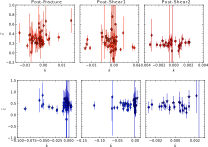
\includegraphics[width=1\columnwidth]{avgRecovBoth_NSPP}
	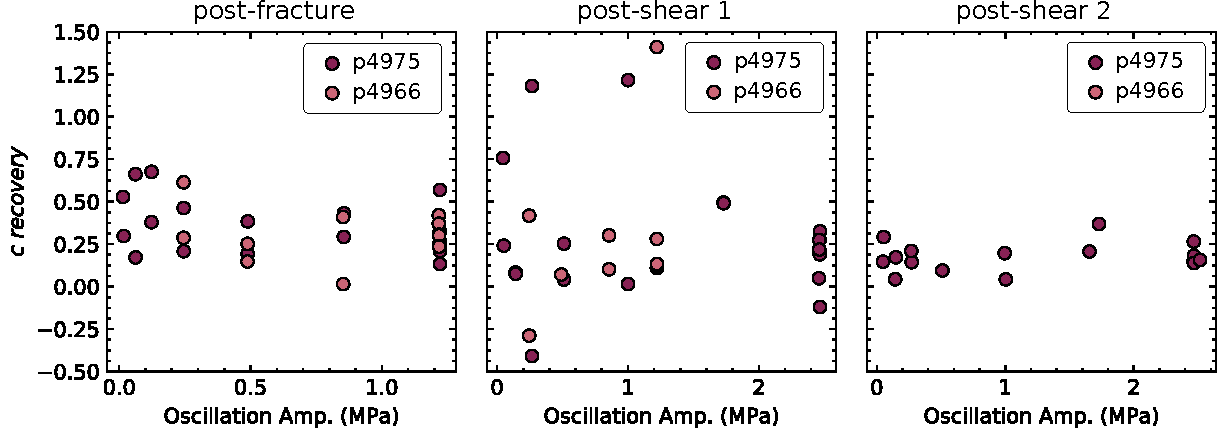
\includegraphics[width=1\columnwidth]{Cdot_NS_amp}
	\includegraphics[width=1\columnwidth]{Cdot_PP_amp}
	%\enspace
	%\includegraphics[width=6cm]{post-frac_amp_array}
	\caption{Velocity recovery averaged over all receivers ($ \overline {\dot c} $) as a function of oscillation amplitude for NS and PP oscillations. 
	I suspect that the we are not waiting long enough to see a trend like J. Elkhoury and others. His recovery values were ~0.5, which he says is related to the dimensionality of the fracture. Shearing the fracture increases the complexity and maybe changes the slope -- dominated by clogging/moving wear material rather than mated aperture.}
	\label{fig:cdot_amp}
\end{figure}

\newpage


%\begin{figure}[ht]
%	\centering
%	%	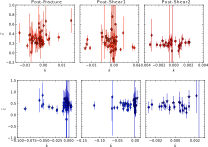
\includegraphics[width=1\columnwidth]{avgRecovBoth_NSPP}
%	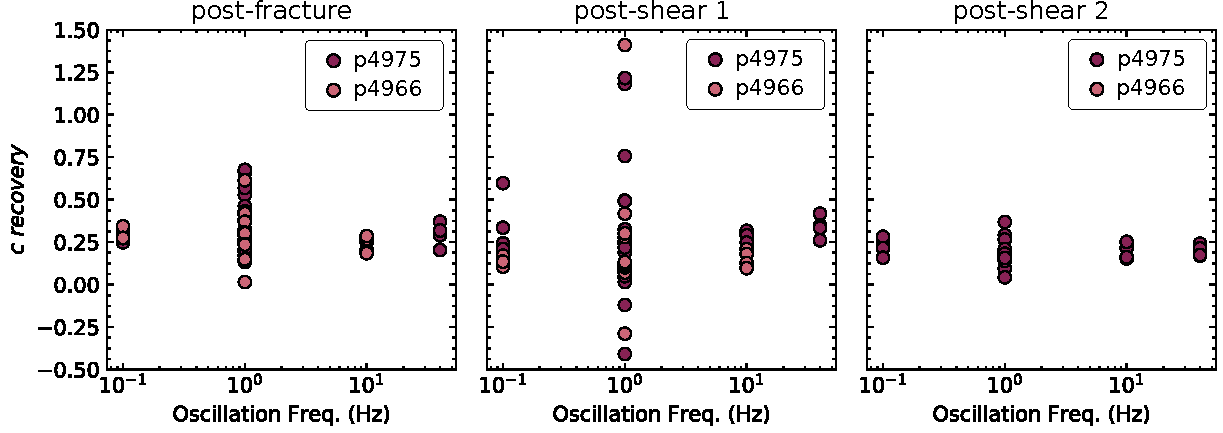
\includegraphics[width=1\columnwidth]{Cdot_NS_freq}
%	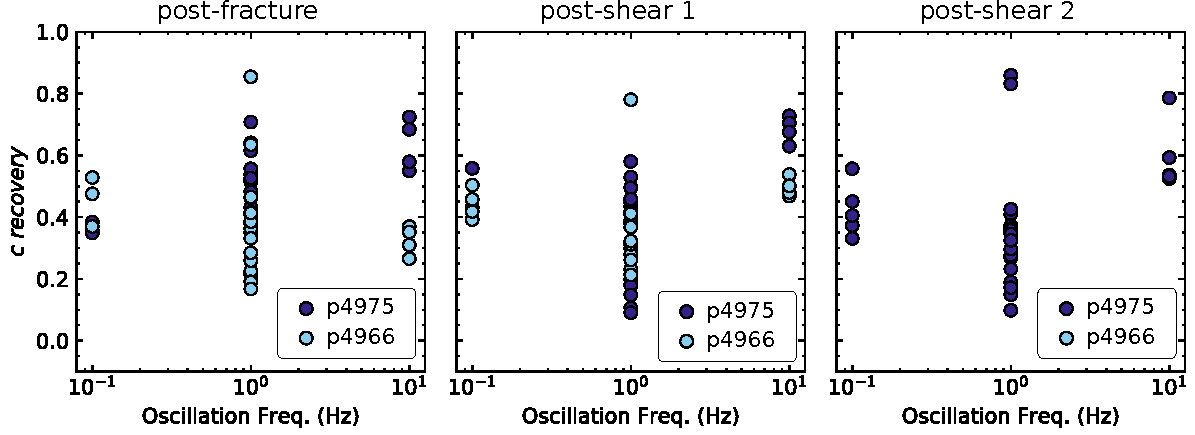
\includegraphics[width=1\columnwidth]{Cdot_PP_freq}
%	%\enspace
%	%\includegraphics[width=6cm]{post-frac_amp_array}
%	\caption{Velocity recovery averaged over all receivers ($ \overline {\dot c} $) as a function of oscillation frequency for NS and PP oscillations. 
%		I suspect that the we are not waiting long enough to see a trend like J. Elkhoury and others. His recovery values were ~0.5, which he says is related to the dimensionality of the fracture. Shearing the fracture increases the complexity and maybe changes the slope -- dominated by clogging/moving wear material rather than mated aperture.}
%	\label{fig:cdot_amp}
%\end{figure}

\newpage

\subsection{Effect of Fracture Aperture}
\begin{itemize}
	\item effect of fracture aperture modulated by shearing the fractured samples in two 5mmincrements, repeating the dynamic stressing protocols. Elucidates how changes in the aperture size distribution due to shearing and wear–alter the fracture stiffness and the stress-dependency.
	\item shearing of the fracture reduces the nonlinearity measured during normal stress oscillations
	\item oscillations become generally less effective in enhancing the fracture permeability.
	\item the correlation between the nonlinearity and permeability change and sample thickness change is stronger for NS oscillations than Pp. 
	\item There is no clear correlation between perm change and flow rate during oscillations, suggesting “unclogging” may not be the sole mechanism responsible for perm change due to Pp oscillations. 
	\item However, we report nonlinearity after the second shear history: indicative of possible differences in mechanisms activated during the two modes of stressing.
\end{itemize}


\section{Supplemental}
\begin{figure}[ht]
	\centering
	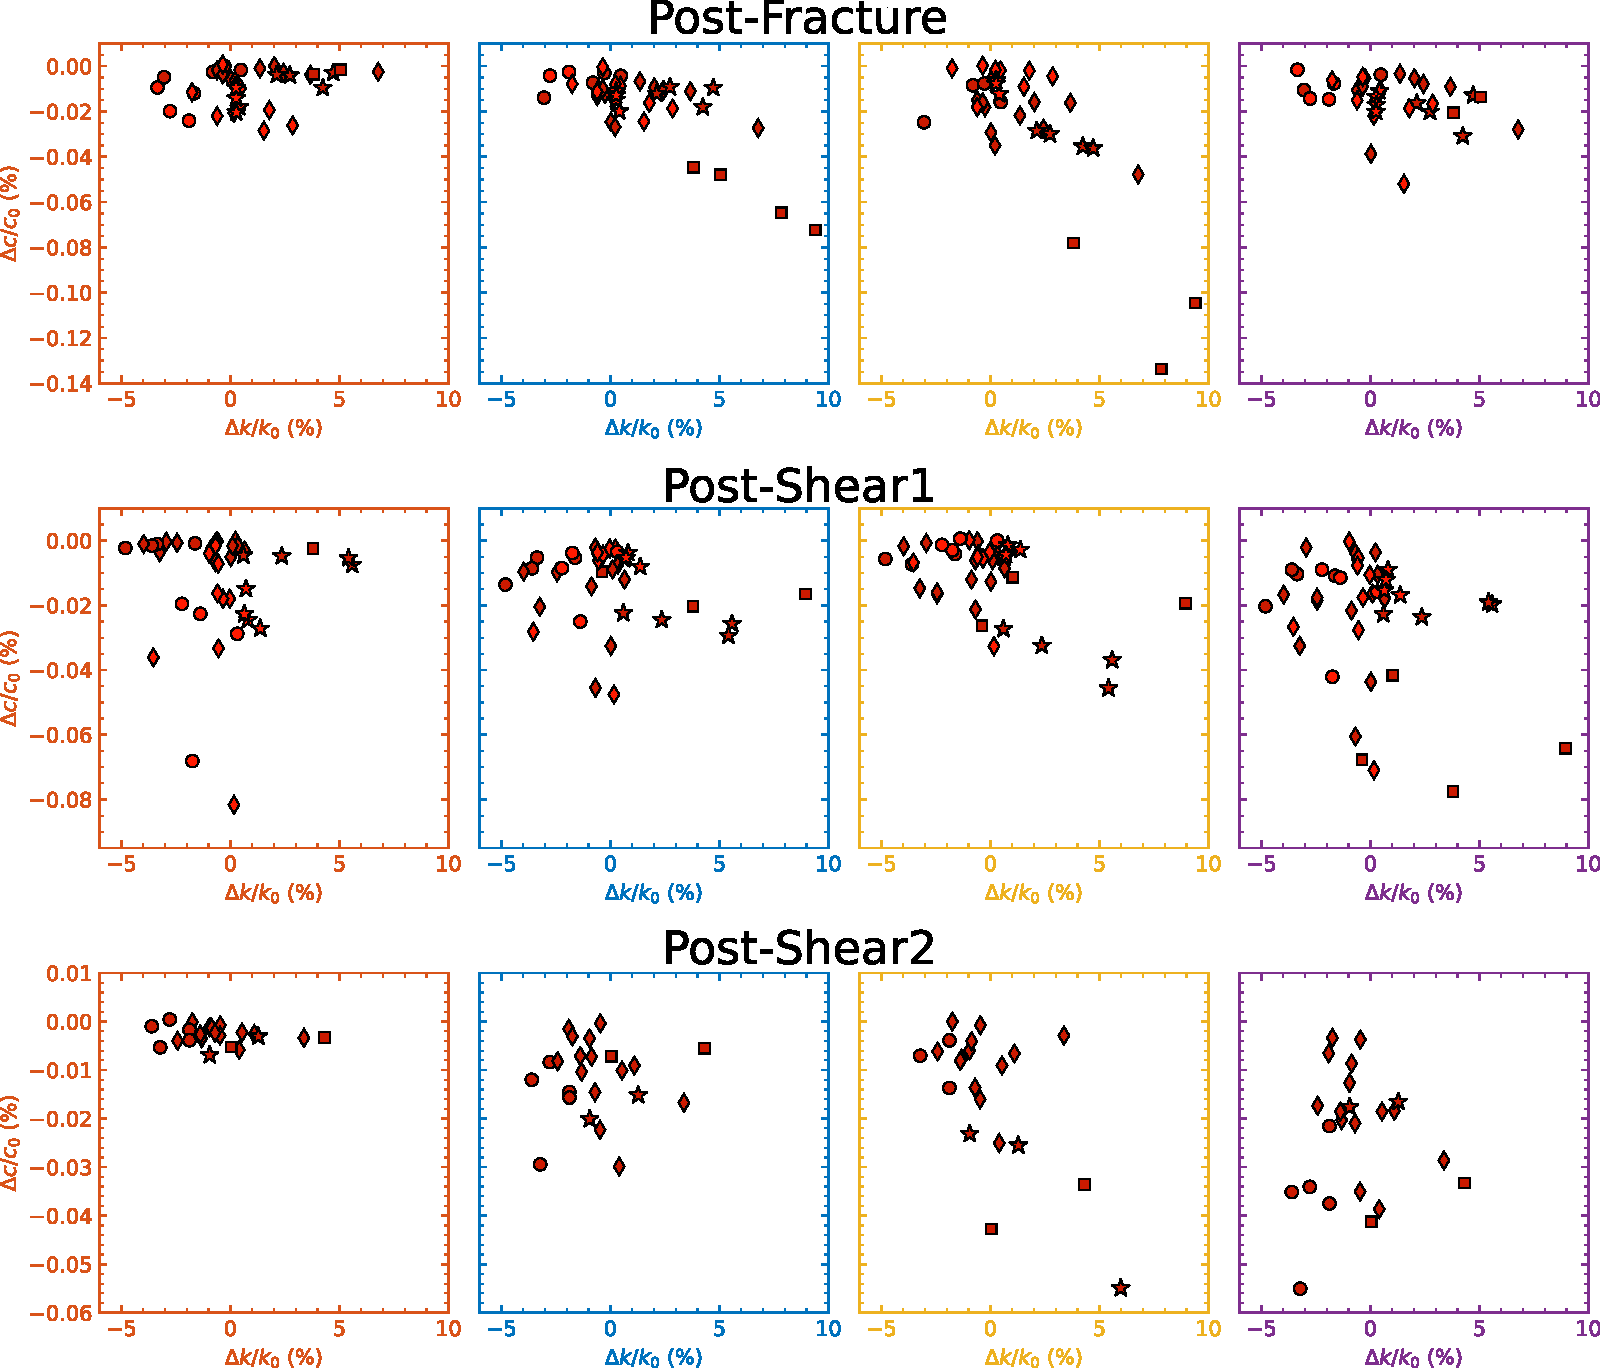
\includegraphics[width=1\columnwidth]{Delc_all_NS_all}
	%\enspace
	%\includegraphics[width=6cm]{post-frac_amp_array}
	\caption{Nonlinearity as a function of permeability change for $ \sigma_{NS} $ oscillations for each receiver. Transitioning from post-fracture results to post-shear results, we observe decreased nonlinearity and permeability enhancement. This is probably related to clogging mechanisms.}%
	\label{fig:delc_plots}
\end{figure}

\newpage

\begin{figure}[ht]
	\centering
	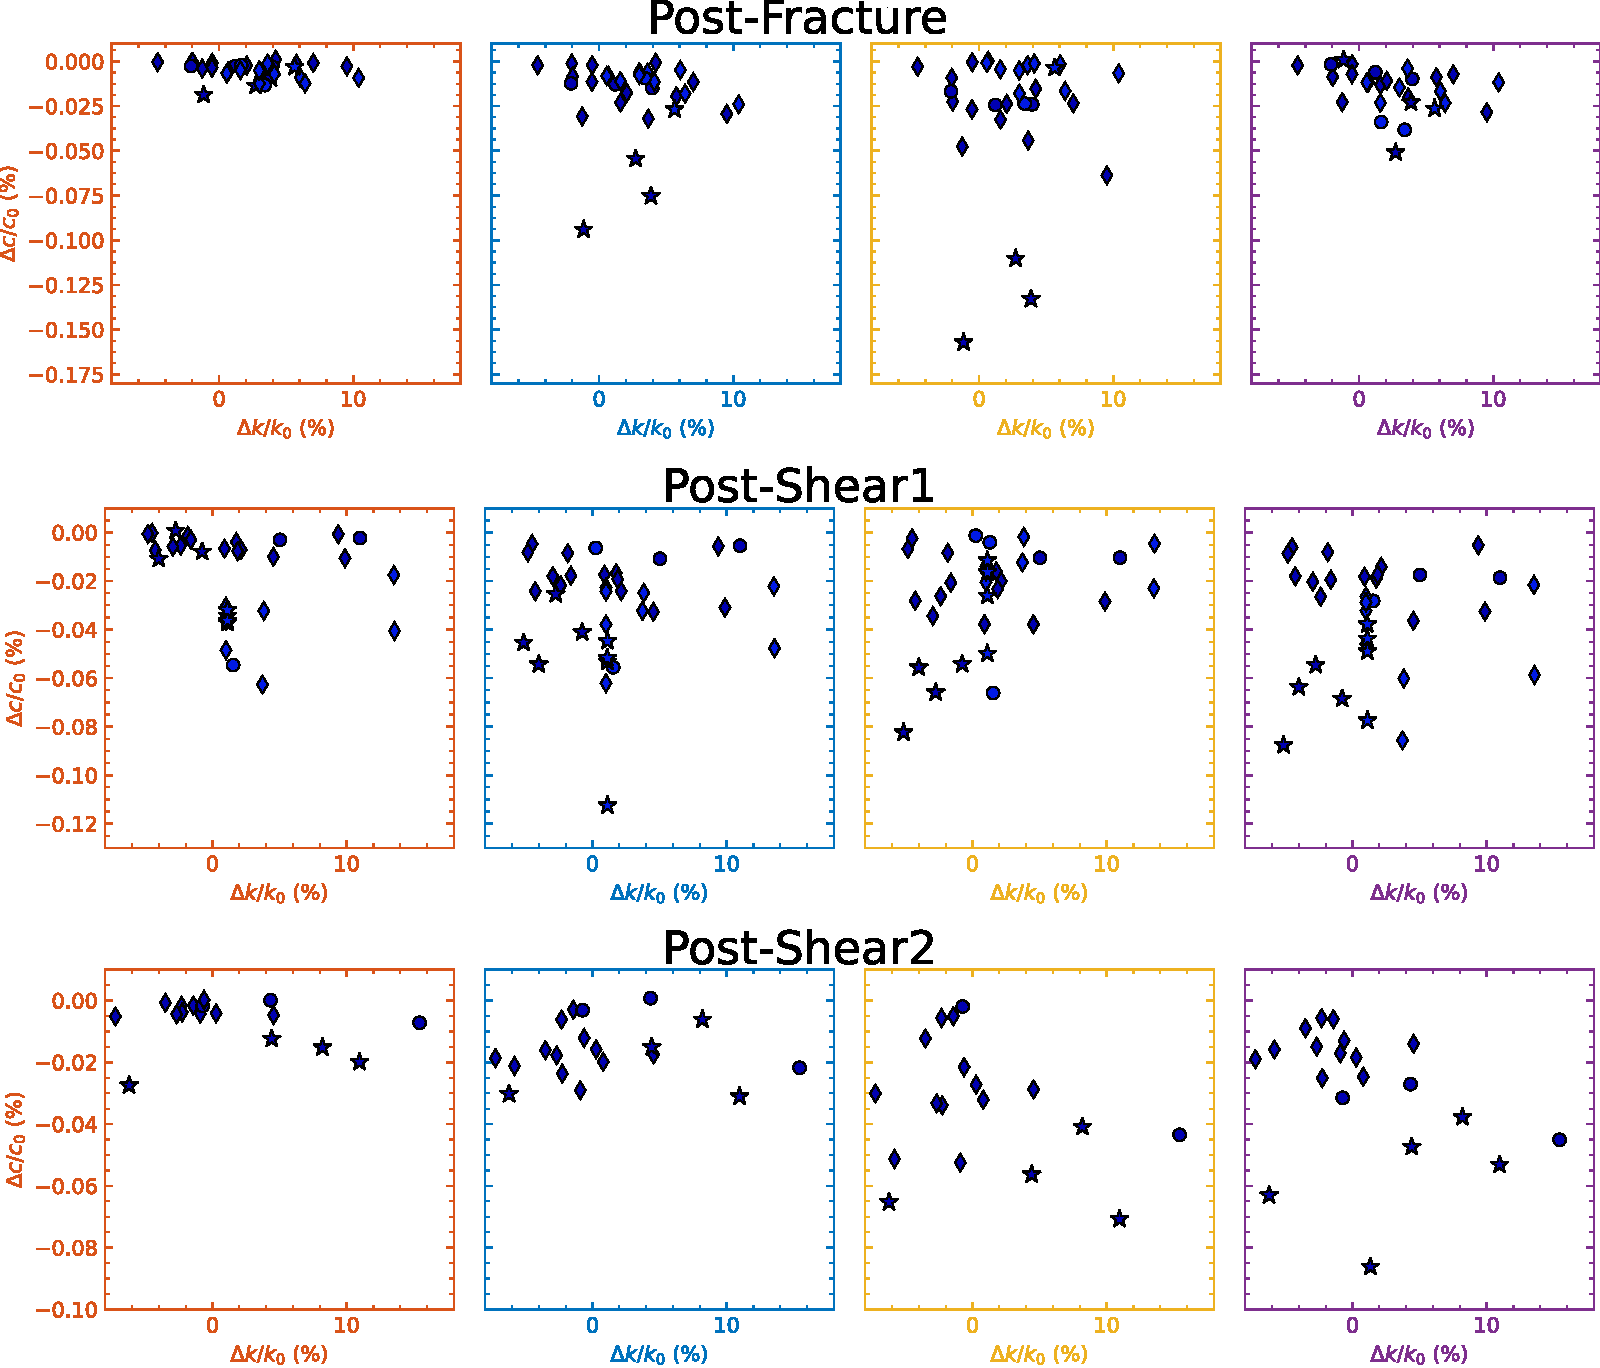
\includegraphics[width=1\columnwidth]{Delc_all_PP_all}
	%\enspace
	%\includegraphics[width=6cm]{post-frac_amp_array}
	\caption{Nonlinearity as a function of permeability change for $ P_P $ oscillations for each receiver.}
	\label{fig:delc_plots2}
\end{figure}

\newpage

%++++++++++++++++++++++++++++++++++++++++
% References section will be created automatically 
% with inclusion of "thebibliography" environment
% as it shown below. See text starting with line
% \begin{thebibliography}{99}
% Note: with this approach it is YOUR responsibility to put them in order
% of appearance.



\end{document}
